\documentclass[12pt,openany]{jbook} 

\usepackage{physics}
\usepackage{amsmath}
\usepackage{amssymb}
\usepackage{amsfonts}

\usepackage[dvipdfmx]{graphicx,xcolor}
\usepackage{hyperref}
\usepackage{listings}
\usepackage{algorithm}
\usepackage{algorithmic}
\usepackage{siunitx}

\renewcommand{\figurename}{図}
\renewcommand{\tablename}{表}
\renewcommand{\algorithmicrequire}{\textbf{Input:}}
\renewcommand{\algorithmicensure}{\textbf{Output:}}
\makeatletter
\renewcommand{\ALG@name}{アルゴリズム}
\makeatother

\usepackage[top=20truemm,bottom=20truemm,left=18truemm,right=18truemm]{geometry}

\usepackage{here}

\usepackage{bm}
\usepackage{amsmath,amssymb}
\usepackage{type1cm}

\usepackage[dvipdfmx]{graphicx}
\usepackage{tikz}

\begin{document}

% 表紙
\begin{center}
    \LARGE{常微分方程式総まとめ}
    
    \Large{\vspace{19cm}にゃにゃん}
    
    \Large{2020年11月12日}
\end{center}
\thispagestyle{empty}
\clearpage

\tableofcontents
\thispagestyle{empty}
\clearpage

% 本文
\pagenumbering{arabic}
\setcounter{page}{1}

\chapter{はじめに}
\label{first}

これは私が微分方程式の解き方を学んでいく中で「この知識を一度体系的にまとめたい」と思って書いたものです。私の持つ知識の範疇で微分方程式の解き方をできる限り体系的にまとめました。

微分方程式を「解く」作業には大きく分けて2つの種類があります。

\begin{itemize}
    \item 解析的に解く
    \item 数値的に解く
\end{itemize}

「解析的に解く」とはつまり、図\ref{fig:1-analytical}\footnote{ここでは簡単のため任意定数は1として考えています。}のように式変形を使用して解くことを言います。ですが世の中に存在する微分方程式のほとんどは今の人類には解析的に解くことができません。そんな中でも様々な工夫をすることで、「この形の微分方程式なら解ける」ということを増やすことができます。

\begin{figure}[ht!]
  \centering
  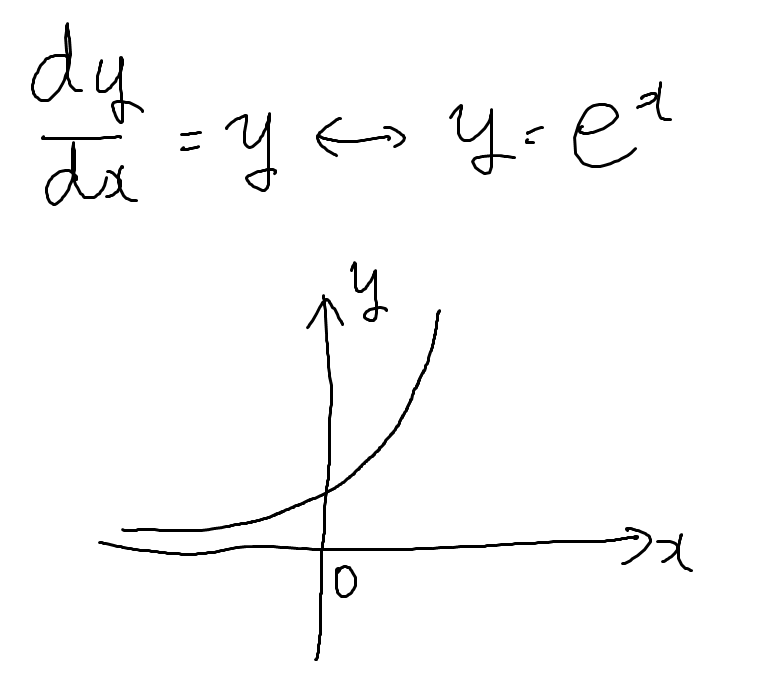
\includegraphics[width=7cm]{img/1-analytical.png}
  \caption{解析的に解く}
  \label{fig:1-analytical}
\end{figure}

「数値的に解く」とは、計算機を用いて微分方程式を近似的に「解く」ことを言います。ここでの「解く」は、何も答えの式が出てくるわけではありません。例えばある$x$における何かの値$y$の数値が、まさに数値として出てくるのです。また、数値的に微分方程式を解いた場合には、求められる解は図\ref{fig:1-numerical}のように離散的(図\ref{fig:1-numerical}ならある決められた値$\Delta x$ごとに$y$が求まります)です。この図についてはこのあと詳しく解説します。

\begin{figure}[ht!]
  \centering
  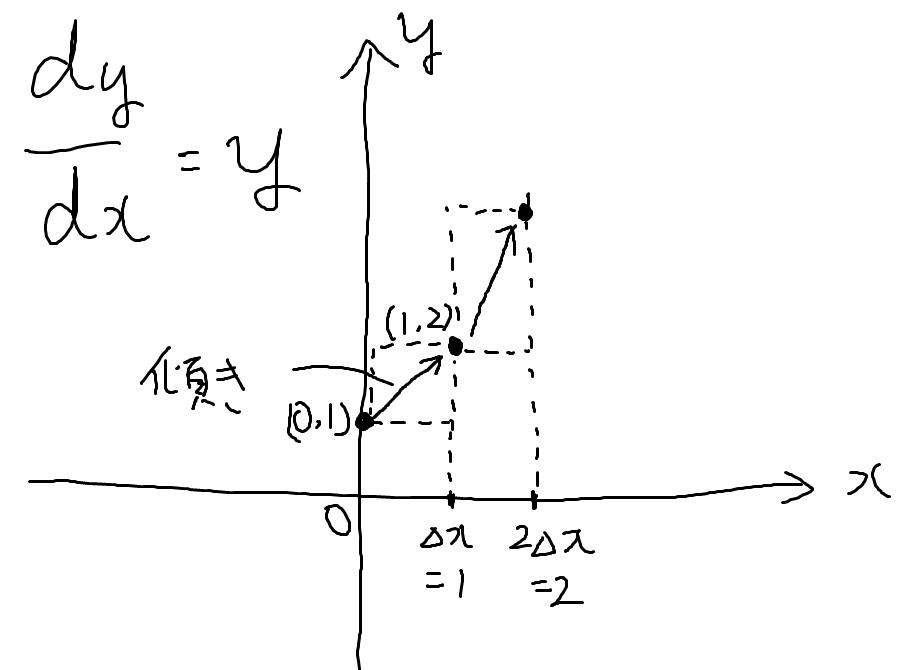
\includegraphics[width=9cm]{img/1-numerical.png}
  \caption{数値的に解く}
  \label{fig:1-numerical}
\end{figure}

本書では微分方程式の解き方についてこの2つの全く異なる方法を解説します。この2つの方法は全く異なるため、便宜上解析的に解く方を先に解説しますが、どちらを先に読んでいただいても構いません。

さて、ここでもう一度図\ref{fig:1-numerical}をご覧ください。これが微分方程式の真髄です。例として出した微分方程式

\begin{eqnarray}
    \frac{\dd y}{\dd x}=y
\end{eqnarray}

\noindent
をもう一度よく睨んでみると……そうです。これは、

\begin{eqnarray}
    (yの傾き)=(yの関数)
\end{eqnarray}

\noindent
という形をしています。「そんなの当たり前じゃないか」と思われる方が大半でしょう。でもよく考えてみてください。ある時点$x$における$y$とそのときの傾きがわかれば、嬉しいことがあります。

\begin{eqnarray}
    y(x+\Delta x)=y(x)+\left.\frac{\dd y}{\dd x}\right|_{x=x}\Delta x
\end{eqnarray}

右辺には既知の値($y$、$\dd y/\dd x$、$\Delta x$)しかありません。そして左辺を見ると、これまでわからなかった$y(x+\Delta x)$が現れています。既知の値を使って未知の値(しかもちょっとだけ$x$が進んだ値)を求める…漸化式みたいですね(実際漸化式の一種だと思います)。

ここで微分方程式の真髄(だと私が思っていること)について一般的な言葉で解説しましょう。

\begin{center}
    「微分方程式はわかっている値を使って「ちょっと先の未来」を知るための方程式である。」
\end{center}

実は解析的に微分方程式を解く場合にはこの真髄が直接役立つことはほぼありません。ですが、「私は今何を解いているのだろう…」と思った時はぜひ思い出してください。「私は未来を知るために微分方程式を解いているのだ」と。

なお、数値的に微分方程式を解くやり方は根本的にこの真髄に従っています。ぜひ覚えておいてください。



\clearpage
\chapter{解析的に常微分方程式を解く}
\label{analytical-ordinary}

第\ref{first}章でも触れた通り、「解析的に微分方程式を解く」とは、式変形を利用して微分方程式を解くことを言います。ですが、世の中にあるほとんどの微分方程式は解析的に解くことができません。でもできれば解析的に微分方程式が解けたほうが様々な考察がしやすくて便利ですよね。ということで人類はできるだけ多くの微分方程式を解析的に解くために様々な技法を考えました。ここでは初歩から込み入った話まで、微分方程式を解析的に解く解き方についてお話しします。







\section{微分の逆操作}
\label{integrate}
まず一番単純な微分方程式を解いてみましょう。こちらの$x$を関数として求めたいとします。
\begin{eqnarray}
    \frac{\dd y}{\dd x}=ax+b
\end{eqnarray}

$a$と$b$は定数です。これをまず見つめてみましょう。何を意味するでしょうか。

\begin{itemize}
    \item $y$の傾きは$x$に比例する
    \item $y$は微分すると$x$のみの関数になる
\end{itemize}

この2点に気づけましたでしょうか。「何を当たり前な」とおっしゃらず、まずは一度考えてみてください。結論から言ってしまえば、これは$y$を微分したものが$x$のみの関数になるので簡単に解くことができます。どうやって解いたら良いでしょうか。こう書いた方がわかりやすいかもしれません。

\begin{eqnarray}
    \label{eq:integrate}
    y'=ax+b
\end{eqnarray}

\noindent
そうです。$y'$から$y$を求めるのであれば単純に両辺積分すれば良いのです。

\begin{eqnarray}
    y&=&\int(ax+b)\dd x \\
    &=&\frac{1}{2}ax^2+bx+C
\end{eqnarray}

ここで、新たに出てきた$C$(言ってしまえばただの積分定数ですが)を「任意定数」と言います。今後は$C$や$A$を用いて任意定数を表すことにします。この任意定数の数はその微分方程式に出てくる微分項の階数の最大値と一致します。任意定数がこの数だけ入った形の解を「一般解」と言います。それに対して例えば今回であれば$y(0)=1$などとして$C=1$と決まったときの解を「特殊解」または「特解」と言います。特殊解を決めるときに使う条件を「初期条件」と言います。「初期」とは言っても必ずしも$x=0$の場合を考える必要はありません。

はい、これでこの微分方程式が解けてしまいました。微分方程式は基本的に積分操作を用いて解きます。そもそも微分の逆操作は積分でしたね。微分された形の方程式を解くのであればそれに積分を使うことはご納得いただけることでしょう。

両辺積分して解くことができる微分方程式の一般形は以下です。

\begin{eqnarray}
    \frac{\dd y}{\dd x}=f(x)
\end{eqnarray}







\section{変数分離形}
\label{separation}
セクションの名前は置いておいて、第\ref{first}章の例として出した微分方程式の少し一般化して定数$k$をつけたもの

\begin{eqnarray}
    \frac{\dd y}{\dd x}=ky
\end{eqnarray}

\noindent
を考えてみましょう。これは式\ref{eq:integrate}と違って右辺に$x$がいるのが厄介そうです。

とりあえずこの式の意味するところを考えてみましょう。

\begin{itemize}
    \item $y$の傾きは$y$に比例する
    \item $y$を微分しても元の$x$の定数倍である
\end{itemize}

この2点に気づけましたでしょうか。1つ目は第\ref{first}章でお話しした「真髄」に関するものです。そして2つ目は式の形をよく睨んで考えついたものです。$y$が増えれば増えるほど$y$の傾きが大きくなる。$y$は微分しても(定数を除いて)形が変わらない。この2点をよく考えると、$y$は指数関数ではないか?という考えが浮かぶでしょう。

このように、まず微分方程式をよく見て求める関数のグラフや、関数の数式としての形を推測することが検算の役に立ちます。

では解いていきましょう。まずは$ky$を左辺に移動させます。

\begin{eqnarray}
    \frac{1}{ky}\frac{\dd y}{\dd x}=1
\end{eqnarray}

\noindent
そして$\dd x$を右辺に移動させ\footnote{「$\dd y/\dd x$は分数ではないのにこんなに軽々しく移動させて良いのか」と疑問の方もいらっしゃるでしょう。実はこれは本来置換積分の式です。$\dd x$を右辺に移動させずに両辺$x$で積分してみましょう。 \\
$\int\frac{1}{ky}\frac{\dd y}{\dd x}\dd x=\int\dd x$ \\
左辺は見慣れた置換積分の式になりましたね。これを形式的に「$\dd x$を右辺に移動させてインテグラルをつける」としています}

\begin{eqnarray}
    \label{eq:separation}
    \frac{1}{ky}\dd y=\dd x
\end{eqnarray}

\noindent
積分してみましょう。

\begin{eqnarray}
    \int\frac{1}{ky}\dd y=\int\dd x \\
    \frac{1}{k}\ln y = x+C
\end{eqnarray}

\noindent
あれれ、$y=$の形では出てきませんでしたね。でもご心配なさらず。このように式変形しましょう。

\begin{eqnarray}
    \ln y&=&kx+kC \nonumber\\
    y&=&e^{kx+kC} \nonumber\\
    y&=&Ae^{kx}
\end{eqnarray}

\noindent
ここで、$A=e^{kC}$としました。$A$と$C$は任意定数です。これで$y=$の形で関数が求められましたね!確かに$y$は指数関数になりました。

さて、いきなりですがこのような方法を「変数分離」と言います。式\ref{eq:separation}をご覧ください。左辺には$y$だけ、右辺には$x$だけが出てくるように「変数を分離」しています。このように、変数を分離できれば両辺をうまく積分することができるようになります。この方法を「変数分離」、変数分離できる形の微分方程式を「変数分離形」と言います。

変数分離形の一般的な形は以下の通りです。

\begin{eqnarray}
    \label{eq:separation-basic}
    \frac{\dd y}{\dd x}=f(x)g(y)
\end{eqnarray}

\noindent
これを、

\begin{eqnarray}
    \int \frac{1}{g(y)}\dd y=\int f(x)\dd x
\end{eqnarray}

\noindent
とすることで、この微分方程式を解くことができます。なお、$g(y)$が恒等的に0の場合は$g(y)$で割ることができません\footnote{「$g(y)$が一瞬でも0を通る場合はどうなんだ」という鋭いツッコミをされる方もいらっしゃるでしょう。結論から言えば大丈夫です。$g(y_0)=0$となる$y_0$が存在するとしましょう。\\
$\frac{\dd y}{\dd x}=f(x)\cdot 0$ \\
となり、右辺が0なので定数関数$y=y_0$は明らかにこの微分方程式の解ですね。ではそれ以外の解を考えてみましょう。定数関数$y=y_0$以外の解で、ある値$y=y_0$を通ることがあるとまずいです。一瞬$g(y)=0$となる関数$g(y)$で除算していることになります。しかし、「解の一意性」を考えるとこのようなことはありません。定数関数$y=y_0$以外の関数$y$である値$y=y_0$を通るとすると、この2つの関数$y$は$xy$座標で描いた際に交差、または接していることになります。ここで初期条件$x=x_0$で$y=y_0$を考えてみましょう。あれれ、どちらの関数を解として良いかわからなくなってしまいましたね。どちらの関数も$(x_0, y_0)$を通ります。このようなことがないことを保証するのが「解の一意性」です。微分方程式の解である関数$y$は互いに交差や接触をしないのです。ですので、ある点$y=y_0$で$g(y_0)=0$となる$g(y)$があったとしても、定数関数$y=y_0$だけ別に考えれば良いというわけです。しかも、この定数関数$y=y_0$は、導いた一般解の関数$y$に含まれます。例えば$y=Ae^{kx}$であれば$k=0$の場合ですね。ですので、結論としては恒等的に0となる関数$g$以外であれば何も考えずに割ってしまって良いのです。}。というか、そもそも右辺自体が恒等的に0になってしまうので全く別の微分方程式になってしまいますね。






\section{同次形}
\label{homogeneous}
さて、ここからどんどん微分方程式を解いていきます。これからはまず微分方程式の一般的な形を示して、その後にその微分方程式を解いていきます。

「同次形」という形の微分方程式の一般形は以下です。
\begin{eqnarray}
    \frac{\dd y}{\dd x}=f\pqty{\frac{y}{x}}
\end{eqnarray}

\noindent
$u=y/x$として$\dd u/\dd x$を計算してみると、

\begin{eqnarray}
    \frac{\dd u}{\dd x}=-\frac{y}{x^2}+\frac{1}{x}\frac{\dd y}{\dd x}
\end{eqnarray}

\noindent
となります。ここから後の式変形のために$\dd y/\dd x$を取り出すと、

\begin{eqnarray}
    \frac{\dd y}{\dd x}=\frac{\dd u}{\dd x}x+u
\end{eqnarray}

\noindent
となります。これを元の微分方程式の左辺に代入して少し変形してみましょう。右辺は$y/x$を$u$に置換します。

\begin{eqnarray}
    \frac{\dd u}{\dd x}x+u&=&f(u) \\
    \frac{\dd u}{\dd x}&=&\frac{1}{x}(f(u)-u)
\end{eqnarray}

\noindent
おっと、これは変数分離形ではないでしょうか。変数分離形の基本形は式\ref{eq:separation-basic}の通りでした。これの$y$を$u$に置換して見ると、右辺は$x$の関数と$u$の関数の積で書いてあることがわかるでしょう。実際に変数分離で解いてみます。

\begin{eqnarray}
    \int \frac{\dd u}{f(u)-u}&=&\int\frac{\dd x}{x}
\end{eqnarray}

このように積分を実行することで、$u$が求められます。$u=y/x$でしたから、求まった$u$に$x$を掛けてやれば求めたい関数$y$が無事求められます。







\subsection{発展版同次形}
\label{advanced-homogeneous}

次に以下の形を考えてみましょう。

\begin{eqnarray}
    \frac{\dd y}{\dd x}=f\pqty{\frac{ax+by+c}{a'x+b'y+c'}}
\end{eqnarray}

\noindent
これも実は同次形に帰着して解くことができます。やってみましょう。

天下り的ですが、

\begin{eqnarray}
    c&=&-a\alpha-b\beta \\
    c'&=&-a'\alpha-b'\beta
\end{eqnarray}

\noindent
を満たす$\alpha$と$\beta$を見つけます。式変形すれば、

\begin{eqnarray}
    \alpha&=&\frac{b'c-bc'}{a'b+ab'} \\
    \beta&=&\frac{-a'c-ac'}{a'b+ab'}
\end{eqnarray}

\noindent
ということがわかると思います。

ここで、$x=X+\alpha$、$y=Y+\beta$と置換します。関数$f$の中の分子は、$c$と$\alpha$、$\beta$の変換式を使えば、

\begin{eqnarray}
    ax+by+c&=&a(X+\alpha)+b(Y+\beta)+c \nonumber \\
    &=&(aX+bY)+(a\alpha+b\beta)+(-a\alpha-b\beta) \nonumber \\
    &=&aX+bY
\end{eqnarray}

\noindent
とすっきりした形になります。分母も同様に、

\begin{eqnarray}
    a'x+b'y+c'=a'X+b'Y
\end{eqnarray}

\noindent
となります。

微分方程式の左辺については、

\begin{eqnarray}
    \frac{\dd y}{\dd x}=\frac{\dd Y}{\dd X}
\end{eqnarray}

\noindent
ですから、結局すべてをまとめると

\begin{eqnarray}
    \frac{\dd Y}{\dd X}=f\pqty{\frac{aX+bY}{a'X+b'Y}}
\end{eqnarray}

\noindent
となります。大分見通しが良くなりましたね。この分子分母をそれぞれ$X$で割ってみましょう。

\begin{eqnarray}
    \frac{\dd Y}{\dd X}=f\pqty{\frac{a+b\frac{Y}{X}}{a'+b'\frac{Y}{X}}}
\end{eqnarray}

出てきました、$Y/X$。これで同次形に帰着できました。あとは\ref{homogeneous}節の同次形として解けます。







\section{一階線形微分方程式}
\label{first-order}
「一階線形微分方程式」とは、以下の形をした微分方程式のことです。

\begin{eqnarray}
    \frac{\dd y}{\dd x}+P(x)y+Q(x)=0
    \label{eq:first-order}
\end{eqnarray}

「一階」とは、微分項の最大階数が1であるという意味、「線形」とは、$\dd y/\dd x$と$y$の線形結合で書かれた方程式であるということを意味します。

このとき、$Q(x)$の状態によってさらに2通りに分けられます。

\begin{itemize}
    \item $Q(x)=0$: 一階斉次線形微分方程式
    \item $Q(x)\neq0$: 一階非斉次線形微分方程式
\end{itemize}

斉次のときは

\begin{eqnarray}
    \frac{\dd y}{\dd x}=-P(x)y
\end{eqnarray}

\noindent
ですから、変数分離形(\ref{separation}節)として解くことができます。解は、

\begin{eqnarray}
    \int \frac{\dd y}{y}=-\int P(x)\dd x \\
    y=Ce^{-\int P(x)\dd x}
    \label{eq:homogeneous-2}
\end{eqnarray}

\noindent
と与えられます。

問題は非斉次のときです。非斉次の場合は2通りの解き方があります。






\subsection{特殊解を見つける}
\label{special-solution}
この微分方程式を満たす特殊解を(エスパーで)発見できれば、あっさりと解くことができます。$y=y_1(x)$はこの微分方程式を満たす特殊解であるとしましょう。

\begin{eqnarray}
    \frac{\dd y_1}{\dd x}+P(x)y_1+Q(x)=0
    \label{eq:special-y_1}
\end{eqnarray}

\noindent
です。ここで、関数$Y(x)$を使って$y=Y+y_1$と置換してみましょう。

\begin{eqnarray}
    \frac{\dd}{\dd x}(Y+y_1)+P(x)(Y+y_1)+Q(x)=0 \\
    \frac{\dd Y}{\dd x}+P(x)Y+\pqty{\frac{\dd y_1}{\dd x}+P(x)y_1+Q(x)}=0 \nonumber \\
    \frac{\dd Y}{\dd x}+P(x)Y=0
\end{eqnarray}

\noindent
式\ref{eq:special-y_1}を使うことで、$Q(x)$の項を消すことができます。これで斉次に帰着できました。変数分離形(\ref{separation}節)として解くことができます。解は、

\begin{eqnarray}
    y=y_1(x)+Ce^{-\int P(x)\dd x}
    \label{eq:homogeneous-special}
\end{eqnarray}

\noindent
です。







\subsection{定数変化法}
\label{constant-change}
微分方程式が簡単な形をしている場合には特殊解をすぐに見つけられることがありますが、そう簡単にはいかない場合もあります。そんなときには定数変化法を使って特殊解を求めましょう。定数変化法は、式\ref{eq:homogeneous-2}の任意定数$C$を$x$の関数であると見て、

\begin{eqnarray}
    y_1=C(x)e^{-\int P(x)\dd x}
    \label{eq:constant-change}
\end{eqnarray}

\noindent
と特殊解を置いて、元の微分方程式に代入して解を探します\footnote{「そんな身勝手なことをして良いのか」という話ですが、これは特殊解を探す一つの手段です。特殊解はどんな関数であれこの微分方程式を満たしてくれさえすれば良いのです。今回はこのような形で特殊解があることを仮定して探します。}。

\begin{eqnarray}
    \frac{\dd}{\dd x}\pqty{C(x)e^{-\int P(x)\dd x}}+P(x)C(x)e^{-\int P(x)\dd x}+Q(x)=0
\end{eqnarray}

\noindent
左辺第一項を実際に微分してみましょう。

\begin{eqnarray}
    \pqty{\frac{\dd}{\dd x}C(x)\cdot e^{-\int P(x)\dd x}-P(x)C(x)e^{-\int P(x)\dd x}}+P(x)C(x)e^{-\int P(x)\dd x}+Q(x)&=&0 \nonumber\\
    \frac{\dd}{\dd x}C(x)\cdot e^{-\int P(x)\dd x}+Q(x)&=&0
\end{eqnarray}

鮮やかに$P(x)C(x)e^{-\int P(x)\dd x}$が打ち消し合って消えてくれました。しかも$Q(x)$は$x$のみの関数で、$C(x)$の関数ではありません。これで$C(x)$を求められそうです。

\begin{eqnarray}
    \frac{\dd}{\dd x}C(x)\cdot e^{-\int P(x)\dd x}&=&-Q(x) \\
    C(x)&=&-\int Q(x)e^{\int P(x)\dd x}\dd x
    \label{eq:constant-change-C}
\end{eqnarray}

これで特殊解が求められました。特殊解$y_1$は、

\begin{eqnarray}
    y_1=-e^{-\int P(x)\dd x}\int Q(x)e^{\int P(x)\dd x}\dd x
\end{eqnarray}

\noindent
です。では\ref{special-solution}節の方法を使って一般解を求めてみましょう。一般解は式\ref{eq:homogeneous-special}を使って、

\begin{eqnarray}
    y&=&-e^{-\int P(x)\dd x}\int Q(x)e^{\int P(x)\dd x}\dd x+Ce^{-\int P(x)\dd x} \nonumber \\
    &=&\pqty{C-\int Q(x)e^{\int P(x)\dd x}\dd x}e^{-\int P(x)\dd x}
    \label{eq:constant-change-ans}
\end{eqnarray}

\noindent
です。なお、ここで出てきた$C$は、紛らわしいですが特殊解を探す上で使用した$C(x)$とは別物で、任意定数です。

ここで、式\ref{eq:constant-change-C}をもう一度見てみましょう。この積分定数(これも一種の微分方程式(\ref{integrate}節で紹介したものに当たります)なので任意定数と言えます)はどこへ行ったのでしょうか。「特殊解を探す」という目的なら積分定数は何でも良いのですが、仮にこれを明示的に$C$と置いてみましょう。ここでも積分定数(任意定数)$C$と関数$C(x)$は別物です。

\begin{eqnarray}
    C(x)=-\int Q(x)e^{\int P(x)\dd x}\dd x+C
\end{eqnarray}

\noindent
これを式\ref{eq:constant-change}に代入すると、

\begin{eqnarray}
    y=\pqty{C-\int Q(x)e^{\int P(x)\dd x}\dd x}e^{-\int P(x)\dd x} \nonumber
\end{eqnarray}

あれ、式\ref{eq:constant-change-ans}(定数変化法を使って求めた一般解)と一致しましたね。実は左辺を特殊解を表す$y_1$でなく一般解を表す$y$にさりげなく置き換えておきました。

一般解はその微分方程式の階数だけの任意定数を含んだものを言います。今回は$C(x)$を求めたときに明示的に積分定数を$C$としたことで、これが任意定数となってしまったのです。

定数変化法は「特殊解を見つける」手段ではありますが、このように任意定数を途中で置いてしまうことで一般解の導出まで一気にできてしまいます。






\subsection{積分因子}
\label{first-order--integrating-factor}
突然ですが問題の式\ref{eq:first-order}の両辺に$e^{\int P(x)\dd x}$を掛けてみましょう。すると、

\begin{eqnarray}
    e^{\int P(x)\dd x}\frac{\dd y}{\dd x}+P(x)e^{\int P(x)\dd x}y+e^{\int P(x)\dd x}Q(x)=0
\end{eqnarray}

となります。左辺第一項、第二項をよく見ると、この2つはまとめて$ye^{\int P(x)\dd x}$の微分の形になっていることに気づきます。

\begin{eqnarray}
    \frac{\dd}{\dd x}\pqty{ye^{\int P(x)\dd x}}+Q(x)e^{\int P(x)\dd x}=0 \nonumber \\
    \frac{\dd}{\dd x}\pqty{ye^{\int P(x)\dd x}}=-Q(x)e^{\int P(x)\dd x}
\end{eqnarray}

右辺は$x$だけの式です。\ref{integrate}節のように両辺を$x$で積分してみましょう。


\begin{eqnarray}
    ye^{\int P(x)\dd x}&=&-\int Q(x)e^{\int P(x)\dd x} \dd x+C \nonumber \\
    y&=&\pqty{C-\int Q(x)e^{\int P(x)\dd x}\dd x}e^{-\int P(x)\dd x}
\end{eqnarray}

狐につままれたような感覚ですが、なんと答えが求まってしまいました。

このように、微分方程式全体にある因子を掛けることで呆気なく微分方程式が解けてしまうことがあります。このような因子を「積分因子」と言います。







\section{完全形}
\label{perfect}

完全形とは、

\begin{eqnarray}
    \frac{\dd y}{\dd x}=-\frac{f(x,y)}{g(x,y)}
    \label{eq:perfect}
\end{eqnarray}

\noindent
という形の微分方程式において、

\begin{eqnarray}
    \frac{\partial f}{\partial y}=\frac{\partial g}{\partial x}
    \label{eq:perfect-terms}
\end{eqnarray}

\noindent
を満たす微分方程式を言います。

これを少し変形してみましょう。\ref{eq:perfect}の分母を払って移項すると、

\begin{eqnarray}
    f(x,y)\dd x+g(x,y)\dd y=0
    \label{eq:perfect-flat}
\end{eqnarray}

\noindent
となります。ここで関数$u(x,y)$を

\begin{eqnarray}
    \frac{\partial u}{\partial x}=f(x,y),\ \frac{\partial u}{\partial y}=g(x,y)
    \label{eq:perfect-u-terms}
\end{eqnarray}

\noindent
と定義して導入します。すると、式\ref{eq:perfect-flat}は、

\begin{eqnarray}
    \frac{\partial u}{\partial x}\dd x+\frac{\partial u}{\partial y}\dd y=0=\dd u
\end{eqnarray}

となります。関数$u$の全微分の形ですね。これが完全形の正体です\footnote{この関数$u$が存在する条件が式\ref{eq:perfect-terms}です}。これを満たす関数$u$を求めれば、それは$x$と$y$の関係が求められたことになるので、「微分方程式が解けた」と言えます\footnote{微分方程式は必ずしも解が$y=$の形にならないといけないわけではありません。$y=$の形になればすっきりしますが、とにかく$x$と$y$の関係が微分項を含まずに記述できればOKなのです。}。

では具体的に関数$u$を求めていきましょう。まずは式\ref{eq:perfect-u-terms}の関数$f$に関する式を積分します。

\begin{eqnarray}
    \frac{\partial u}{\partial x}&=&f(x,y) \nonumber \\
    u&=&\int f(x,y) \dd x+h(y)
    \label{eq:perfect-ans-u}
\end{eqnarray}

\noindent
元々$x$で偏微分した形で書かれた式を積分したので、関数$h(y)$が出てきます。$\int f(x,y) \dd x$は与えられた式を積分するだけなので良いとして、問題はこの関数$h$です。とりあえず式\ref{eq:perfect-u-terms}の関数$g$に関する式に代入して関数$h$について整理してみましょう。

\begin{eqnarray}
    \frac{\partial}{\partial y}\pqty{\int f(x,y) \dd x+h(y)}=g(x,y) \\
    \frac{\dd }{\dd y}h(y)=g(x,y)-\frac{\partial}{\partial y}\int f(x,y) \dd x
    \label{eq:perfect-u}
\end{eqnarray}

両辺を$y$で積分してみると、

\begin{eqnarray}
    h(y)=\int\pqty{g(x,y)-\frac{\partial}{\partial y}\int f(x,y) \dd x}\dd y
\end{eqnarray}

\noindent
となります。ここで両辺をよく睨むと、左辺の関数$h$は$y$のみの関数なのに、右辺には$x$の関数が2つ出てくることに気づくでしょう。つまり、右辺の$x$を含む項は互いに打ち消し合っているのです。少し寄り道して、この$g(x,y)-\int f(x,y) \dd x$を$x$で偏微分して値が本当に0になるか($x$を含む項が打ち消し合っているか)を見てみましょう。

\begin{eqnarray}
    \frac{\partial}{\partial x}\pqty{g(x,y)-\frac{\partial}{\partial y}\int f(x,y) \dd x}&=&\frac{\partial g}{\partial x}-\frac{\partial f}{\partial y}
\end{eqnarray}

式\ref{eq:perfect-terms}の条件を考えると、確かに右辺は0になります。

さて、では本筋に戻りましょう。$\partial/\partial y\int f(x,y) \dd x$についてよく考えてみましょう。式\ref{eq:perfect-u}で積分定数(定数ではなく関数ですが)を$h(y)$と置いたので、$\int f(x,y) \dd x$単体には今積分定数(関数)がありません。つまり、この全ての項には$x$が何らかの形でつきます。これを$y$で偏微分したところで、全ての項に$x$が関わることに変わりはありません。つまり上の議論の通り、$\partial/\partial y\int f(x,y) \dd x$に出てくる項は全て$g(x,y)$と打ち消し合ってしまうのです。

ここから以下が言えます。

\begin{eqnarray}
    h(y)=\int g(x,y)\dd y\ \mbox{に出てくる$x$を含まない項}
\end{eqnarray}

さて、$g(x,y)$は与えられた式ですので、これを$y$で積分して適宜$y$を含む項を抜き去れば$h(y)$が求められるということになります。なんとこれを式\ref{eq:perfect-ans-u}に代入すれば、目的の関数$u$は求まってしまいます。数式としてこれを記述し直すと、

\begin{eqnarray}
    u(x,y)=\int f(x,y)\dd x+\int \pqty{g(x,y)-\frac{\partial}{\partial y}\pqty{\int g(x,y)\dd x}}\dd y
    \label{eq:perfect-ans}
\end{eqnarray}

\noindent
となります。







\subsection{積分因子}
\label{perfect-integrating-factor}
積分因子、再登場です。

\begin{eqnarray}
    \frac{\dd y}{\dd x}=-\frac{f(x,y)}{g(x,y)} \nonumber
\end{eqnarray}

\noindent
という形の微分方程式があっても

\begin{eqnarray}
    \frac{\partial f}{\partial y}=\frac{\partial g}{\partial x} \nonumber
\end{eqnarray}

\noindent
を満たさなければ完全形とは言えません。ですが、右辺の分子分母に$\lambda(x,y)$を掛けることで微分方程式が完全形になる場合があります。この積分因子を見つける系統的な手法はありませんが、積分因子に$x^my^n$を仮定して

\begin{eqnarray}
    \frac{\partial \lambda f}{\partial y}=\frac{\partial \lambda g}{\partial x}
\end{eqnarray}

\noindent
に代入して$m$と$n$を求められる場合があります。








\section{ベルヌーイの微分方程式}
\label{bernoulli}
ここから人名のついた微分方程式が連続します。まずはベルヌーイの微分方程式です。これは、

\begin{eqnarray}
    \frac{\dd y}{\dd x}+f(x)y=g(x)y^n
\end{eqnarray}

\noindent
という形をしたものです。$n=0,1$であれば一階線形微分方程式ですが、ここでは$n\geq2$の場合を考えてみましょう。$z=y^{1-n}$として、まず$\dd z/\dd x$を計算します。

\begin{eqnarray}
    \frac{\dd z}{\dd x}=(1-n)y^{-n}\frac{\dd y}{\dd x}
\end{eqnarray}

微分方程式全体に$(1-n)y^{-n}$を掛けると、

\begin{eqnarray}
    \frac{\dd y}{\dd x}(1-n)y^{-n}+f(x)(1-n)y^{1-n}&=&(1-n)g(x) \\
    \frac{\dd z}{\dd x}+(1-n)f(x)z&=&(1-n)g(x)
\end{eqnarray}

\noindent
となります。これは一階線形微分方程式ですね。\ref{first-order}節の通りに解くことができます。$z$について解を求めて、$y=\sqrt[1-n]{z}$と置換すれば答えが求まります。






\section{リカッチの微分方程式}
\label{ricatch}
リカッチの微分方程式は

\begin{eqnarray}
    \frac{\dd y}{\dd x}=f(x)+g(x)y+h(x)y^2
\end{eqnarray}

の形をしたものです。$f(x)=0$でベルヌーイの微分方程式(\ref{bernoulli}節)です。これは頑張って特殊解$y=y_1(x)$を見つけて、\ref{special-solution}節と同じように関数$Y(x)$を使って$y=Y+y_1$と置きます。まず特殊解の条件を書いておきましょう。

\begin{eqnarray}
    \frac{\dd y_1}{\dd x}=f(x)+g(x)y_1+h(x)y_1^2
    \label{eq:ricatch-terms}
\end{eqnarray}

それでは実際に置換してみましょう。

\begin{eqnarray}
    \frac{\dd Y}{\dd x}+\frac{\dd y_1}{\dd x}&=&f(x)+g(x)(Y+y_1)+h(x)(Y+y_1)^2 \\
    \frac{\dd Y}{\dd x}+\frac{\dd y_1}{\dd x}&=&\pqty{f(x)+g(x)y_1+h(x)y_1^2}+g(x)Y+h(x)Y^2+2h(x)Yy_1
\end{eqnarray}

\noindent
式\ref{eq:ricatch-terms}を使って左辺第二項と右辺のカッコの中を消しましょう。

\begin{eqnarray}
    \frac{\dd Y}{\dd x}&=&g(x)Y+h(x)Y^2+2h(x)Yy_1 \nonumber \\
    &=&(g(x)+2h(x)y_1)Y+h(x)Y^2
\end{eqnarray}

これはベルヌーイの微分方程式($n=2$)です。$z=Y^{-1}$として式全体に$-Y^{-2}$を掛けると、

\begin{eqnarray}
    -Y^{-2}\frac{\dd Y}{\dd x}&=&-(g(x)+2h(x)y_1)Y^{-1}-h(x) \nonumber \\
    \frac{\dd z}{\dd x}&=&-(g(x)+2h(x)y_1)z-h(x)
\end{eqnarray}

これで一階線形微分方程式に帰着できました。\ref{first-order}節の方法を使って解くことができます。$z$について解いて$y=y_1+1/z$と置換すれば答えが求まります。







\section{ダランベールの微分方程式}
\label{dalambert}
ダランベールの微分方程式はこんな形をしています。

\begin{eqnarray}
    y=xf\pqty{\frac{\dd y}{\dd x}}+g\pqty{\frac{\dd y}{\dd x}}
\end{eqnarray}

$\dd y/\dd x$を$p$と置いて両辺を$x$で微分してみましょう。

\begin{eqnarray}
    \label{eq:dalambert-y}
    y&=&xf(p)+g(p) \\
    p&=&f(p)+x\frac{\dd p}{\dd x}\frac{\dd}{\dd p}f(p)+\frac{\dd p}{\dd x}\frac{\dd}{\dd p}g(p)
\end{eqnarray}

\noindent
少しトリッキーですが、ここで$\dd x/\dd p$についてまとめてみましょう。つまり、$x$を$p$の関数と見るということです。

\begin{eqnarray}
    \pqty{x\frac{\dd}{\dd p}f(p)+\frac{\dd}{\dd p}g(p)}\frac{\dd p}{\dd x}&=&p-f(p) \\
    \frac{\dd x}{\dd p}&=&\frac{\frac{\dd}{\dd p}f(p)}{p-f(p)}x+\frac{\frac{\dd}{\dd p}g(p)}{p-f(p)}
\end{eqnarray}

これは$x$と$p$の一階線形微分方程式です。$x$を$p=\dd y/\dd x$について解きます。すると、

\begin{eqnarray}
    x=h(p)
\end{eqnarray}

\noindent
という関数$h(p)$を伴った式が現れます。これと式\ref{eq:dalambert-y}を連立することで$p$を消去します。言わば$p$を媒介変数として$y$と$x$の関係を求めるわけですね。







\subsection{クレローの微分方程式}
\label{clairaut}
クレローの微分方程式はダランベールの微分方程式の特殊な場合です。

\begin{eqnarray}
    y=x\frac{\dd y}{\dd x}+g(\frac{\dd y}{\dd x})
\end{eqnarray}

\noindent
ダランベールの微分方程式で$f(\dd y/\dd x)=\dd y/\dd x$となったものですね。ダランベールの微分方程式と同じように$p=\dd y/\dd x$を導入して両辺を$x$で微分してみましょう。

\begin{eqnarray}
    \label{eq:clairaut-y}
    y&=&xp+g(p) \\
    p&=&p+x\frac{\dd p}{\dd x}+\frac{\dd p}{\dd x}\frac{\dd}{\dd p}g(p) \\
    0&=&\frac{\dd p}{\dd x}\pqty{x+\frac{\dd}{\dd p}g(p)}
\end{eqnarray}

\noindent
かなりすっきりしましたね。左辺が0ですので、右辺の2項のどちらが0になるかで場合分けしましょう。

\begin{itemize}
    \item $\dd p/\dd x=0$のとき、$p=C$より$y=Cx+g(C)$です。この場合が特殊です。
    \item $x+\dd g(p)/\dd p=0$のとき、これと式\ref{eq:clairaut-y}を連立して$p$を消去して解となります。この場合はただのダランベールの微分方程式ですね。
\end{itemize}










\section{二階線形微分方程式}
\label{second-order}
二階の微分項が入った形の微分方程式です。

\begin{eqnarray}
    \frac{\dd^2y}{\dd x^2}+P(x)\frac{\dd y}{\dd x}+Q(x)y+R(x)=0
\end{eqnarray}

これについて、一階線形微分方程式と同様に斉次・非斉次の場合の大まかな解き方をご説明しましょう。

$R(x)=0$、つまり斉次の場合は、階数である2つの線形独立な解($y=y_2,y=y_3$\footnote{本書では$y_1$を特殊解の意味で使っているので$y_2$から始まるようにしました。少し見にくいですが許してください。}とします。これらを基本解と言います。)\footnote{線形独立でない解とは、ここでは$k$を定数として、$y2=ky_3$のように片方がもう片方の定数倍で表すことができる解のことです。つまり、線形独立な解とは片方が片方の定数倍で表せない解のことを言います。}の重ね合わせ(線形結合)

\begin{eqnarray}
    y=c_2y_2+c_3y_3
\end{eqnarray}

\noindent
が一般解です。なお、$c_2$と$c_3$は任意定数です。

この重ね合わせの原理はなぜ成り立つのでしょうか。実際に$y=c_2y_2+c_3y_3$を微分方程式に代入してみましょう。

\begin{eqnarray}
    &&c_2\frac{\dd^2y_2}{\dd x^2}+c_3\frac{\dd^2y_3}{\dd x^2}+c_2P(x)\frac{\dd y_2}{\dd x}+c_3P(x)\frac{\dd y_3}{\dd x}+c_2Q(x)y_2+c_3Q(x)y_3 \nonumber\\
    &=&c_2\pqty{\frac{\dd^2y_2}{\dd x^2}+P(x)\frac{\dd y_2}{\dd x}+Q(x)y_2}+c_3\pqty{\frac{\dd^2y_3}{\dd x^2}+P(x)\frac{\dd y_3}{\dd x}+Q(x)y_3} \nonumber\\
    &=&0 \nonumber
\end{eqnarray}

$y_2$と$y_3$がこの微分方程式を満たすことを利用すれば、確かに$y=c_2y_2+c_3y_3$も解でした。式をよく睨むと、この重ね合わせの原理は微分方程式の線形性\footnote{$y^2$のように$n$乗された項や$y\dd y/\dd x$のように$y$にまつわる関数同士が掛けられた項がないということです。}から来る性質だということがわかります。

ところが、$R(x)\neq0$、つまり非斉次の場合には重ね合わせの原理は成り立ちません。実際に微分方程式に代入して確かめてみてください。非斉次の場合は頑張って特殊解$y=y_1$を見つけ、$y=Y+y_1$と置換して$Y$についての線形独立な2つの基本解$Y=Y_2, Y=Y_3$を見つけます。これらの重ね合わせと$y_1$との和

\begin{eqnarray}
    y=y_1+c_2Y_2+c_3Y_3
\end{eqnarray}

\noindent
が解となります。

もしかしたらお気づきかもしれませんが、一般の$n$階線形微分方程式については$n$個の線形独立な基本解を見つけ、その全ての解を重ね合わせたものが一般解になります。







\subsection{定数係数の二階斉次線形微分方程式}
\label{second-order-const}
定数係数なので、このような形をした微分方程式です。

\begin{eqnarray}
    \frac{\dd^2y}{\dd x^2}+a\frac{\dd y}{\dd x}+by=0
    \label{eq:second-order-const}
\end{eqnarray}

右辺が0でないときは非斉次です。特殊解$y=y_1$を探して斉次に持ち込みましょう。このとき、定数変化法が使えます。\ref{second-order-constant-change}節でお話しします。

斉次式(右辺$=0$)の場合は解に

\begin{eqnarray}
    y=e^{\lambda x}
    \label{eq:second-order-const-y}
\end{eqnarray}

\noindent
の形を仮定して微分方程式に代入してみます\footnote{「解を仮定なんてして良いのか」と思われるかもしれませんが、私たちがやるべきことはどんな形の解であれ線形独立な基本解を2つ見つけることです。仮定した解がうまく本当の解になってくれたら嬉しくありませんか?}。すると、

\begin{eqnarray}
    \lambda^2e^{\lambda x}+a\lambda e^{\lambda x}+be^{\lambda x}&=&0 \\
    \lambda^2+a\lambda+b&=&0
    \label{eq:second-order-lambda}
\end{eqnarray}

\noindent
という二次方程式になります。これを特性方程式と言います。なんだかとてもすっきりしましたね。この判別式の正負で場合分けをしましょう。



\subsubsection{判別式が正の場合}
判別式が正とは、

\begin{eqnarray}
    a^2-4b>0
\end{eqnarray}

\noindent
のときのことを言います。この場合、$\lambda$について、2つの実数解$\lambda_2, \lambda_3$\footnote{ここも特殊解との区別、およびインデックスを揃えるために2で始まるようにしています}が求まります。この場合、それぞれの$\lambda$を式\ref{eq:second-order-const-y}に代入すると、線形独立な2つの基本解が求まります。片方がもう片方の定数倍で表せることはありません。よって、一般解は

\begin{eqnarray}
    y=c_2e^{\lambda_2x}+c_3e^{\lambda_3x}
\end{eqnarray}

\noindent
です。

\subsubsection{判別式が負の場合}
判別式が負なので、

\begin{eqnarray}
    a^2-4b<0
\end{eqnarray}

\noindent
の場合です。こちらも$\lambda$について2つの複素数解$\lambda_2, \lambda_3$が求まります。このままこの$\lambda$を式\ref{eq:second-order-const-y}に代入すれば2つの基本解が求まります。よって、一般解は判別式が正の場合と同じく

\begin{eqnarray}
    y=c_2e^{\lambda_2x}+c_3e^{\lambda_3x} \nonumber
\end{eqnarray}

\noindent
です。

\subsubsection{判別式が0の場合}
問題は判別式が0の場合です。

\begin{eqnarray}
    a^2-4b=0
    \label{eq:second-order-same}
\end{eqnarray}

二次方程式の解$\lambda_2$が重解となって1つしか現れません。そこで、定数変化法を使ってみましょう。2つの基本解を以下のように置いてみます。$y_2$は出てきた$\lambda_2$をそのまま式\ref{eq:second-order-const-y}に入れた形です。

\begin{eqnarray}
    y_2&=&e^{\lambda_2 x} \\
    y_3&=&C(x)e^{\lambda_2 x}
    \label{eq:second-order-const-y3}
\end{eqnarray}

これがもし解になれば、$C(x)$は$x$の関数なので、線形独立な基本解が求められることになります。これを元の微分方程式\ref{eq:second-order-const}に代入してみるのですが、その前に$\dd y_3/\dd x$と$\dd^2 y_3/\dd x^2$を求めておきましょう。

\begin{eqnarray}
    \frac{\dd y_3}{\dd x}&=&e^{\lambda_2 x}\pqty{\frac{\dd}{\dd x}C(x)+\lambda_2 C(x)} \\
    \frac{\dd^2 y_3}{\dd x^2}&=&\lambda_2 e^{\lambda_2 x}\pqty{\frac{\dd}{\dd x}C(x)+\lambda_2 C(x)}+e^{\lambda_2 x}\pqty{\frac{\dd^2}{\dd x^2}C(x)+\lambda_2 \frac{\dd}{\dd x}C(x)} \nonumber \\
    &=&e^{\lambda_2 x}\pqty{\frac{\dd^2}{\dd x^2}C(x)+2\lambda_2 \frac{\dd}{\dd x}C(x)+\lambda_2^2C(x)}
\end{eqnarray}

では式\ref{eq:second-order-const}に代入しましょう。

\begin{eqnarray}
    e^{\lambda_2 x}\pqty{\frac{\dd^2}{\dd x^2}C(x)+2\lambda_2 \frac{\dd}{\dd x}C(x)+\lambda_2^2C(x)}+ae^{\lambda_2 x}\pqty{\frac{\dd}{\dd x}C(x)+\lambda_2 C(x)}+bC(x)e^{\lambda_2 x}=0 \\
    \pqty{\frac{\dd^2}{\dd x^2}C(x)+2\lambda_2 \frac{\dd}{\dd x}C(x)+\lambda_2^2C(x)}+a\pqty{\frac{\dd}{\dd x}C(x)+\lambda_2 C(x)}+bC(x)=0 \nonumber \\
    \frac{\dd^2}{\dd x^2}C(x)+(2\lambda_2+a)\frac{\dd}{\dd x}C(x)+(\lambda_2^2+a\lambda_2+b)C(x)=0
\end{eqnarray}

左辺が恒等的に0でなくてはいけないのです。$C(x)$の項は、式\ref{eq:second-order-lambda}より、$C(x)$の係数が0になります。

次に$\dd C(x)/\dd x$の項を考えますが、ここで重解$\lambda$を$a$を使って表しましょう。判別式の条件式\ref{eq:second-order-same}と$\lambda$の特性方程式\ref{eq:second-order-lambda}より、

\begin{eqnarray}
    \lambda=-\frac{1}{2}a
    \label{eq:second-order-lambda-same}
\end{eqnarray}

\noindent
です。よって、

\begin{eqnarray}
    (2\lambda+a)\frac{\dd}{\dd x}C(x)=0
\end{eqnarray}

\noindent
です(左辺第一項が0になります)。

残ったのは$\dd C(x)/\dd x$だけですね。よって、

\begin{eqnarray}
    \frac{\dd^2}{\dd x^2}C(x)=0
\end{eqnarray}

\noindent
が成り立ちます。

定数変化法の根本的な条件$C(x)\neq0$を考えれば、

\begin{eqnarray}
    C(x)=kx
\end{eqnarray}

ということが導けます。ここでは定数$k$は何でも良いので、1として、

\begin{eqnarray}
    C(x)=x
\end{eqnarray}

\noindent
としておきましょう。

元の話に戻ると、結局2つの線形独立な基本解は式\ref{eq:second-order-const-y3}に$C(x)=x$を代入すれば、

\begin{eqnarray}
    y_2&=&e^{\lambda_2 x} \nonumber\\
    y_3&=&xe^{\lambda_2 x}
\end{eqnarray}

\noindent
となります。よって、一般解$y$は、

\begin{eqnarray}
    y=(c_2+c_3x)e^{\lambda_2 x}
\end{eqnarray}

\noindent
です。








\subsection{定数係数の二階非斉次線形微分方程式}
\label{second-order-constant-change}

非斉次なので、式\ref{eq:second-order-const}の右辺を$f(x)$とします。

\begin{eqnarray}
    \frac{\dd^2y}{\dd x^2}+a\frac{\dd y}{\dd x}+by=f(x)
    \label{eq:second-order-const-nhm}
\end{eqnarray}

方針としては、特殊解$y=y_1$を見つけ、$y=Y+y_1$と置換して$Y$を求めるのですが、今回は先に斉次式を解きます。斉次式

\begin{eqnarray}
    \frac{\dd^2Y}{\dd x^2}+a\frac{\dd Y}{\dd x}+by=0
\end{eqnarray}

\noindent
の一般解$Y=C_2Y_2+C_3Y_3$を求めたとします。ここで定数変化法です。特殊解$y_1$もこの一般解と似ているだろうと仮定して、

\begin{eqnarray}
    y_1=c_2(x)Y_2+c_3(x)Y_3
\end{eqnarray}

と置いてみます。では実際に微分方程式に代入するために、$\dd y_1/\dd x$と$\dd^2 y_2/\dd x^2$を求めてみましょう。

\begin{eqnarray}
    \frac{\dd y_1}{\dd x}=\frac{\dd}{\dd x}c_2(x)Y_2+c_2(x)\frac{\dd Y_2}{\dd x}+\frac{\dd}{\dd x}c_3(x)Y_3+c_3(x)\frac{\dd Y_3}{\dd x}
\end{eqnarray}

ちょっと待ってください。これをもう一度微分したい気持ちにはなれませんね。ということで都合よくこんな条件を付け加えてみましょう。

\begin{eqnarray}
    \frac{\dd}{\dd x}c_2(x)Y_2+\frac{\dd}{\dd x}c_3(x)Y_3=0
    \label{eq:second-order-const-nhm-terms}
\end{eqnarray}

どんな都合の良い条件を加えようと、とにかく特殊解が見つかれば良いのです。今回の微分方程式だとこのようにして特殊解を見つけられます。

この条件によって、

\begin{eqnarray}
    \frac{\dd y_1}{\dd x}&=&c_2(x)\frac{\dd Y_2}{\dd x}+c_3(x)\frac{\dd Y_3}{\dd x} \\
    \frac{\dd^2 y_1}{\dd x^2}&=&\pqty{\frac{\dd}{\dd x}c_2(x)}\frac{\dd Y_2}{\dd x}+c_2(x)\frac{\dd^2 Y_2}{\dd x^2}+\pqty{\frac{\dd}{\dd x}c_3(x)}\frac{\dd Y_3}{\dd x}+c_3(x)\frac{\dd^2 Y_3}{\dd x^2}
\end{eqnarray}

\noindent
となります。では元の微分方程式\ref{eq:second-order-const-nhm}に代入してみましょう。

\begin{eqnarray}
    \pqty{\frac{\dd}{\dd x}c_2(x)}\frac{\dd Y_2}{\dd x}+c_2(x)\frac{\dd^2 Y_2}{\dd x^2}+\pqty{\frac{\dd}{\dd x}c_3(x)}\frac{\dd Y_3}{\dd x}+c_3(x)\frac{\dd^2 Y_3}{\dd x^2} \nonumber \\
    +a\pqty{c_2(x)\frac{\dd Y_2}{\dd x}+c_3(x)\frac{\dd Y_3}{\dd x}}+b(c_2(x)Y_2+c_3(x)Y_3)=f(x)
\end{eqnarray}

2行に渡る式になってしまいましたが怯まずに整理しましょう。

\begin{eqnarray}
    c_2(x)\pqty{\frac{\dd^2 Y_2}{\dd x^2}+a\frac{\dd Y_2}{\dd x}+bY_2}+c_3(x)\pqty{\frac{\dd^2 Y_3}{\dd x^2}+a\frac{\dd Y_3}{\dd x}+bY_3} \nonumber \\
    +\pqty{\frac{\dd}{\dd x}c_2(x)}\frac{\dd Y_2}{\dd x}+\pqty{\frac{\dd}{\dd x}c_3(x)}\frac{\dd Y_3}{\dd x}=f(x)
\end{eqnarray}

$Y_1,Y_2$はそれぞれ斉次方程式の解だったので、上段がばっさり0になり、

\begin{eqnarray}
    \pqty{\frac{\dd}{\dd x}c_2(x)}\frac{\dd Y_2}{\dd x}+\pqty{\frac{\dd}{\dd x}c_3(x)}\frac{\dd Y_3}{\dd x}=f(x)
\end{eqnarray}

となります。これとさきほどの都合よくつけた成約条件式\ref{eq:second-order-const-nhm-terms}をあわせて連立方程式を解きます。その際、行列を使うとこんな風に書けます。

\begin{eqnarray}
    \left(
        \begin{array}{cc}
            Y_2 & Y_3 \\
            \frac{\dd Y_2}{\dd x} & \frac{\dd Y_3}{\dd x}
        \end{array}
    \right)
    \left(
        \begin{array}{c}
            \frac{\dd}{\dd x}c_2(x) \\
            \frac{\dd}{\dd x}c_3(x)
        \end{array}
    \right)
    =
    \left(
        \begin{array}{c}
            0 \\
            f(x)
        \end{array}
    \right)
\end{eqnarray}

随分すっきりしましたね。この行列の両辺に左から左辺第一項の行列($W$とします)の逆行列を掛ければ答えが求まりそうです。逆行列の存在確認のために行列$W$の行列式が0でないことを確認しなくてはならないのですが、実はこの行列$W$には「ロンスキー行列」という名前がついていて、この場合だと$Y_2$と$Y_3$が線形独立であれば行列式は$x$の値によらず絶対に0にはなりません\footnote{ロンスキー行列は一般的に$n$個の関数とその微分が入ったものでもそれぞれが全て線形独立であれば$\det(W)\neq0$です。}。では逆行列を両辺に左から掛けましょう。

\begin{eqnarray}
    \left(
        \begin{array}{c}
            \frac{\dd}{\dd x}c_2(x) \\
            \frac{\dd}{\dd x}c_3(x)
        \end{array}
    \right)
    =
    \frac{1}{Y_2\frac{\dd Y_3}{\dd x}-Y_3\frac{\dd Y_2}{\dd x}}
    \left(
        \begin{array}{cc}
            \frac{\dd Y_3}{\dd x} &-Y_3 \\
            -\frac{\dd Y_2}{\dd x} &Y_2 \\
        \end{array}
    \right)
    \left(
        \begin{array}{c}
            0 \\
            f(x)
        \end{array}
    \right)
\end{eqnarray}

これを$\dd c_2(x)/\dd x$と$\dd c_3(x)/\dd x$のそれぞれについて整理すると、

\begin{eqnarray}
    \frac{\dd}{\dd x}c_2(x)&=&-\frac{Y_3f(x)}{Y_2\frac{\dd Y_3}{\dd x}-Y_3\frac{\dd Y_2}{\dd x}} \\
    \frac{\dd}{\dd x}c_3(x)&=&\frac{Y_2f(x)}{Y_2\frac{\dd Y_3}{\dd x}-Y_3\frac{\dd Y_2}{\dd x}}
\end{eqnarray}

\noindent
となります。これでやっと$c_2(x)$と$c_3(x)$がわかります。それらは、

\begin{eqnarray}
    c_2(x)&=&-\int\frac{Y_3f(x)}{Y_2\frac{\dd Y_3}{\dd x}-Y_3\frac{\dd Y_2}{\dd x}}\dd x \\
    c_3(x)&=&\int\frac{Y_2f(x)}{Y_2\frac{\dd Y_3}{\dd x}-Y_3\frac{\dd Y_2}{\dd x}}\dd x
\end{eqnarray}

\noindent
です。今は特殊解を求めているので積分定数は考えなくて大丈夫です。

これで特殊解が求まりました。よって全体の解は、

\begin{eqnarray}
    y=-Y_2\int\frac{Y_3f(x)}{Y_2\frac{\dd Y_3}{\dd x}-Y_3\frac{\dd Y_2}{\dd x}}\dd x+Y_3\int\frac{Y_2f(x)}{Y_2\frac{\dd Y_3}{\dd x}-Y_3\frac{\dd Y_2}{\dd x}}\dd x+C_2Y_2+C_3Y_3
\end{eqnarray}

\noindent
です。








\subsection{標準形}
\label{basic}
標準形の微分方程式とは、定数$k$を使って

\begin{eqnarray}
    \frac{\dd^2y}{\dd x^2}+ky=0
    \label{eq:basic}
\end{eqnarray}

\noindent
と書ける微分方程式のことです。これは比較的簡単に解くことができます。これを解くのは後に回して、実は一般的な二階斉次線形微分方程式を標準形に帰着することができます。

\begin{eqnarray}
    \frac{\dd^2 y}{\dd x^2}+P(x)\frac{\dd y}{\dd x}+Q(x)y=0
    \label{eq:second-order-normal}
\end{eqnarray}

\noindent
について、

\begin{eqnarray}
    y=u(x)e^{-\frac{1}{2}\int P(x)\dd x}
\end{eqnarray}

\noindent
と置いてみましょう。

\begin{eqnarray}
    \frac{\dd y}{\dd x}&=&\pqty{\frac{\dd}{\dd x}u(x)-\frac{1}{2}P(x)u(x)}e^{-\frac{1}{2}\int P(x)\dd x} \\
    \frac{\dd^2 y}{\dd x^2}&=&\pqty{\frac{\dd^2}{\dd x^2}u(x)-\frac{1}{2}u(x)\frac{\dd}{\dd x}P(x)-\frac{1}{2}P(x)\frac{\dd}{\dd x}u(x)}e^{-\frac{1}{2}\int P(x)\dd x} \nonumber \\
    &-&\frac{1}{2}\pqty{\frac{\dd}{\dd x}u(x)-\frac{1}{2}P(x)u(x)}P(x)e^{-\frac{1}{2}\int P(x)\dd x} \nonumber \\
    &=&\pqty{\frac{\dd^2}{\dd x^2}u(x)-P(x)\frac{\dd}{\dd x}u(x)+\pqty{\frac{1}{4}P^2(x)-\frac{1}{2}\frac{\dd}{\dd x}P(x)}u(x)}e^{-\frac{1}{2}\int P(x)\dd x}
\end{eqnarray}

これを元の微分方程式\ref{eq:second-order-normal}に代入してみます。

\begin{eqnarray}
    \pqty{\frac{\dd^2}{\dd x^2}u(x)-P(x)\frac{\dd}{\dd x}u(x)+\pqty{\frac{1}{4}P^2(x)-\frac{1}{2}\frac{\dd}{\dd x}P(x)}u(x)}e^{-\frac{1}{2}\int P(x)\dd x} \nonumber \\
    +P(x)\pqty{\frac{\dd}{\dd x}u(x)-\frac{1}{2}P(x)u(x)}e^{-\frac{1}{2}\int P(x)\dd x}+Q(x)u(x)e^{-\frac{1}{2}\int P(x)\dd x}=0
\end{eqnarray}

整理すると、

\begin{eqnarray}
    \frac{\dd^2}{\dd x^2}u(x)+\pqty{Q(x)-\frac{1}{2}\frac{\dd}{\dd x}P(x)-\frac{1}{4}P^2(x)}u(x)=0
\end{eqnarray}

\noindent
となります。これで一般的な二階斉次線形微分方程式が標準形になりました。

では実際に標準形の微分方程式\ref{eq:basic}を解いていきましょう。$k$の値によって場合分けができます。

\subsubsection{$k=0$の場合}
微分方程式\ref{eq:basic}を書き直すと

\begin{eqnarray}
    \frac{\dd^2y}{\dd x^2}=0
\end{eqnarray}

\noindent
となるので、$y$の最大の次数は1です。よって、2つの線形独立な基本解を

\begin{eqnarray}
    y_2=x \\
    y_3=1
\end{eqnarray}

\noindent
と置くことができます。よって、これらの重ね合わせを一般解として、一般解は

\begin{eqnarray}
    y=c_2x+c_3
\end{eqnarray}

\noindent
です。

\subsubsection{$k<0$の場合}

微分方程式\ref{eq:basic}を書き直すと、

\begin{eqnarray}
    \frac{\dd^2y}{\dd x^2}=-ky
\end{eqnarray}

\noindent
となりますが、$k$が負なので右辺の係数は正になります。

これは定数係数の二階斉次線形微分方程式ですから、解に$y=e^{\lambda x}$を仮定すると、

\begin{eqnarray}
    \lambda^2e^{\lambda x}=-ke^{\lambda x} \\
    \lambda=\pm \sqrt{-k}
\end{eqnarray}

\noindent
となり、2つの$\lambda$が現れます。これで基本解が2つ作れそうです。基本解$y_2,y_3$は、

\begin{eqnarray}
    y_2&=&e^{\sqrt{-k}x} \\
    y_3&=&e^{-\sqrt{-k}x}
\end{eqnarray}

\noindent
ですので、一般解$y$は

\begin{eqnarray}
    y=c_2e^{\sqrt{-k}x}+c_3e^{-\sqrt{-k}x}
\end{eqnarray}

\noindent
です。

\subsubsection{$k>0$の場合}
微分方程式\ref{eq:basic}を書き直すと、

\begin{eqnarray}
    \frac{\dd^2y}{\dd x^2}=-ky
\end{eqnarray}

\noindent
となります。今回は$k>0$なので右辺の係数は負です。これは見慣れた単振動型の微分方程式ですが一度真面目に解いてみましょう。

これは定数係数の二階斉次線形微分方程式ですから、先ほどと同じように解に$y=e^{\lambda x}$を仮定すると、

\begin{eqnarray}
    \lambda^2e^{\lambda x}=-ke^{\lambda x} \\
    \lambda=\pm i\sqrt{k}
\end{eqnarray}

\noindent
となります。先ほどと同じく2つの$\lambda$が現れたので、線形独立な基本解が2つ作れます。基本解$y_2,y_3$は、

\begin{eqnarray}
    y_2&=&e^{i\sqrt{k}x} \\
    y_3&=&e^{-i\sqrt{k}x}
\end{eqnarray}

\noindent
ですので、一般解$y$は

\begin{eqnarray}
    y=c_2e^{i\sqrt{k}x}+c_3e^{-i\sqrt{k}x}
\end{eqnarray}

\noindent
です。オイラーの公式

\begin{eqnarray}
    e^{i\theta}=\cos\theta+i\sin\theta
\end{eqnarray}

を使えば、

\begin{eqnarray}
    y&=&c_2(\cos\sqrt{k}x+i\sin\sqrt{k}x)+c_3(\cos\sqrt{k}x-i\sin\sqrt{k}x) \nonumber \\
    &=&(c_2+c_3)\cos\sqrt{k}x+i(c_2-c_3)\sin\sqrt{k}x
\end{eqnarray}

となり、$y$が物理量など、解が実数のみを取るという成約があれば、

\begin{eqnarray}
    c_1=\frac{A_1+iA_2}{2} \\
    c_2=\frac{A_1-iA_2}{2}
\end{eqnarray}

\noindent
として、

\begin{eqnarray}
    y=A_1\cos\sqrt{k}x+A_2\sin\sqrt{k}x
\end{eqnarray}

\noindent
です。








\section{演算子の因数分解}
\label{factorization}
$a,b$を定数として微分方程式

\begin{eqnarray}
    \pqty{\frac{\dd^2}{\dd x^2}+(a+b)\frac{\dd}{\dd x}+ab}y=0
\end{eqnarray}

\noindent
を考えてみましょう。演算子をまとめてしまっていますが、定数係数の二階微分方程式です。

この演算子を「因数分解」してしまいましょう。

\begin{eqnarray}
    \pqty{\frac{\dd}{\dd x}+a}\pqty{\frac{\dd}{\dd x}+b}y=0
\end{eqnarray}

これをこんな風に見てしまいます。

\begin{eqnarray}
    \frac{\dd y}{\dd x}+ay=0\ \mbox{または}\ \frac{\dd y}{\dd x}+by=0
\end{eqnarray}

なんと二階の微分方程式が一階の微分方程式になってしまいました。これらの解は変数分離形として見つけられ、この2つの解の線形結合

\begin{eqnarray}
    y=c_1e^{-ax}+c_2e^{-bx}
\end{eqnarray}

\noindent
が解となります。









\section{オイラーの微分方程式}
\label{euler}
オイラーの微分方程式は、

\begin{eqnarray}
    x^2\frac{\dd^2 y}{\dd x^2}+ax\frac{\dd y}{\dd x}+by=0
    \label{eq:euler}
\end{eqnarray}

\noindent
の形をしたものです。解に$y=x^\lambda$を仮定すると、

\begin{eqnarray}
    x^2\lambda(\lambda-1)x^{\lambda-2}+ax\lambda x^{\lambda-1}+bx^\lambda&=&0 \\
    \lambda(\lambda-1)+a\lambda+b&=&0 \nonumber \\
    \lambda^2+(a-1)\lambda+b&=&0
    \label{eq:euler-characteristic}
\end{eqnarray}

\noindent
と、すっきりした形になります。二次方程式が出てきたのでまた決まって判別式で場合分けをします。

\subsubsection{判別式が0でない場合}
判別式に関する条件は

\begin{eqnarray}
    (a-1)^2-4b\neq0
\end{eqnarray}

\noindent
です。この場合は$\lambda$について2つの解$\lambda_2$と $\lambda_3$が求まるため、これらを使った基本解を重ね合わせて

\begin{eqnarray}
    y=c_2x^{\lambda_2}+c_3x^{\lambda_3}
\end{eqnarray}

\noindent
が解です。

\subsubsection{判別式が0の場合}
判別式に関する条件は

\begin{eqnarray}
    (a-1)^2-4b=0
\end{eqnarray}

です。この場合、$\lambda$は1つの重解$\lambda_2$のみを持ちます。2つの基本解がなくてはいけないのに困りましたね。こんなときには定数変化法です。2つの基本解を

\begin{eqnarray}
    y_2&=&x^{\lambda_2} \\
    y_3&=&c(x)x^{\lambda_2}
\end{eqnarray}

\noindent
と置きます。まず$y_3$の微分したものを求めておきます。

\begin{eqnarray}
    \frac{\dd y_3}{\dd x}&=&x^{\lambda_2}\frac{\dd}{\dd x}c(x)+\lambda_2x^{\lambda_2-1}c(x) \\
    \frac{\dd^2 y_3}{\dd x^2}&=&x^{\lambda_2}\frac{\dd^2}{\dd x^2}c(x)+2\lambda_2x^{\lambda_2-1}\frac{\dd}{\dd x}c(x)+\lambda_2(\lambda_2-1)x^{\lambda_2-2}c(x)
\end{eqnarray}

では元の微分方程式\ref{eq:euler}に代入してみましょう。

\begin{eqnarray}
    x^2\pqty{x^{\lambda_2}\frac{\dd^2}{\dd x^2}c(x)+2\lambda_2x^{\lambda_2-1}\frac{\dd}{\dd x}c(x)+\lambda_2(\lambda_2-1)x^{\lambda_2-2}c(x)} \nonumber \\
    +ax\pqty{x^{\lambda_2}\frac{\dd}{\dd x}c(x)+\lambda_2x^{\lambda_2-1}c(x)}+bc(x)x^{\lambda_2}=0
\end{eqnarray}

また2行になってしまいましたが頑張って整理します。定数変化法は総じて計算が煩雑になるので、できればエスパーで求めたいものです…。

\begin{eqnarray}
    x^{\lambda_2+2}\frac{\dd^2}{\dd x^2}c(x)+(2\lambda_2+a)x^{\lambda_2+1}\frac{\dd}{\dd x}c(x)+(\lambda_2^2+(a-1)\lambda_2+b)x^{\lambda_2}c(x)=0
\end{eqnarray}

なんだか\ref{second-order-const}節で見た展開ですが、まず$c(x)$の項の係数が式\ref{eq:euler-characteristic}より0になります。そして、実際に$\lambda_2$を$a$を使った式で求めてみると、

\begin{eqnarray}
    \lambda_2=\frac{1-a}{2}
\end{eqnarray}

\noindent
となるので、式を整理すると、

\begin{eqnarray}
    x^{\lambda_2+2}\frac{\dd^2}{\dd x^2}c(x)+x^{\lambda_2+1}\frac{\dd}{\dd x}c(x)=0 \\
    \frac{\dd^2}{\dd x^2}c(x)=-\frac{1}{x}\frac{\dd}{\dd x}c(x)
\end{eqnarray}

\noindent
となります。この微分方程式は比較的簡単に解けそうです。まず$\dd c(x)/\dd x=c'(x)$を求めることを考えると、これは変数分離形です。

\begin{eqnarray}
    \frac{\dd}{\dd x}c'(x)&=&-\frac{1}{x}c'(x) \\
    \int \frac{1}{c'(x)}\dd c'(x)&=&-\int\frac{1}{x}\dd x \nonumber \\
    \ln|c'(x)|&=&-\ln|x| \nonumber \\
    c'(x)&=&\pm\frac{1}{x}
\end{eqnarray}

\noindent
これを$x$で積分すれば、

\begin{eqnarray}
    c(x)=\ln|x|
\end{eqnarray}

\noindent
このように$c(x)$が求まります。よって2つの線形独立な基本解は、

\begin{eqnarray}
    y_2&=&x^{\lambda_2} \nonumber \\
    y_3&=&x^{\lambda_2}\ln|x|
\end{eqnarray}

一般解は、

\begin{eqnarray}
    y=x^{\lambda_2}(c_2+c_3\ln|x|)
\end{eqnarray}

\noindent
です。










\section{定数係数連立微分方程式}
\label{multiple}
こんな微分方程式が与えられたとします。

\begin{eqnarray}
y_1&=&y \nonumber \\
\frac{\dd y_1}{\dd x}&=&y_2 \nonumber \\
\frac{\dd y_2}{\dd x}&=&y_3 \nonumber \\
\vdots \nonumber\\
\frac{\dd y_n}{\dd x}&=&f(x,y_1,...,y_{n-1})
\end{eqnarray}

これを行列を使った式にしてみましょう。

\begin{eqnarray}
    \boldsymbol{y}&=&(y_1,y_2,...,y_n) \\
    A&=&\pqty{\begin{array}{ccc}
        a_{1\ 1} & \hdots & a_{1\ n} \\
        \vdots & \ddots & \vdots \\
        a_{n\ 1} & \hdots & a_{n\ n}
    \end{array}}
\end{eqnarray}

\noindent
を導入して、行列$A$の要素を適当に決めると微分方程式が

\begin{eqnarray}
    \frac{\dd \boldsymbol{y}}{\dd x}=A\boldsymbol{y}
    \label{eq:multiple-y}
\end{eqnarray}

\noindent
と表せます。この$\boldsymbol{y}$がベクトルではなかった場合は、解が何になったでしょうか。$y=e^{\lambda x}$でしたね。今回は$\boldsymbol{c}$を任意定数で構成された定ベクトルとして、

\begin{eqnarray}
    \boldsymbol{y}=\boldsymbol{c}e^{A x}
\end{eqnarray}

\noindent
と解を置いてみましょう。

行列$A$の$n$個の固有値を$\lambda_1,\lambda_2,\cdots,\lambda_n$、固有ベクトルを$\boldsymbol{p}_1,\boldsymbol{p}_2,\cdots,\boldsymbol{p}_n$とすると、解は

\begin{eqnarray}
    \boldsymbol{y}=c_1e^{\lambda_1 x}\boldsymbol{p}_1+c_2e^{\lambda_2 x}\boldsymbol{p}_2+\cdots+c_ne^{\lambda_n x}\boldsymbol{p}_n
\end{eqnarray}

\noindent
です。






\section{級数展開法}
\label{expansion}
微分方程式の解として級数解が求まる場合があります。与えられた微分方程式に

\begin{eqnarray}
    y=\sum_{n=0}^\infty c_n(x-a)^n
\end{eqnarray}

\noindent
を仮定して代入します。テイラー展開の形ですね。例として一階の微分方程式\ref{eq:first-order}

\begin{eqnarray}
    \frac{\dd y}{\dd x}+P(x)y+Q(x)=0 \nonumber
\end{eqnarray}

\noindent
を考えると、

\begin{eqnarray}
    \sum_{n=0}^\infty nc_n(x-a)^{n-1}+P\pqty{\sum_{n=0}^\infty c_n(x-a)^n}+Q(x)=0
\end{eqnarray}

\noindent
となり、$x$の次数に注目して両辺の係数を比較することで$i$番目の$c_i$が求まる場合があります。この方法を整級数展開法と言います。

「求まる場合がある」と書いたのは、例えば0でない定数$\alpha$を使って

\begin{eqnarray}
c_i=c_i+\alpha
\end{eqnarray}

\noindent
となるなど、$c_i$が求まらない場合があるのです。この場合は求める関数$y$が$x=a$周りでテイラー展開できません。

具体的な級数解の求め方は本節の小節で紹介します。








\subsection{正則点と特異点・フロベニウスの方法}
\label{regular-singular}
二階斉次線形微分方程式

\begin{eqnarray}
    \frac{\dd^2 y}{\dd x^2}+P(x)\frac{\dd y}{\dd x}+Q(x)y=0
\end{eqnarray}

\noindent
について、場合分けをします。

\begin{itemize}
    \item $P(x),Q(x)$が$x=a$でなめらか: $x=a$は正則点
    \item 上でなく、$(x-a)P(x),(x-a)^2Q(x)$が$x=a$でなめらか: $x=a$は確定特異点
    \item それ以外: $x=a$は不確定特異点
\end{itemize}

正則点周りの展開は整級数展開で答えが得られます。

確定特異点周りは$c_0\neq0$として、解を

\begin{eqnarray}
    y&=&\sum_{n=0}^\infty c_n(x-a)^{n+\lambda}
\end{eqnarray}

\noindent
と置きます。微分すると、

\begin{eqnarray}
    \frac{\dd y}{\dd x}&=&\sum_{n=0}^\infty c_n(n+\lambda)(x-a)^{n+\lambda-1} \\
    \frac{\dd^2 y}{\dd x^2}&=&\sum_{n=0}^\infty c_n(n+\lambda)(n+\lambda-1)(x-a)^{n+\lambda-2}
\end{eqnarray}

\noindent
です。また、$P(x)$と$Q(x)$について、

\begin{eqnarray}
    (x-a)P(x)=\sum_{n=0}^\infty p_n(x-a)^n \\
    (x-a)^2Q(x)=\sum_{n=0}^\infty q_n(x-a)^n
\end{eqnarray}

\noindent
と展開することにします。すると、与えられた微分方程式は

\begin{eqnarray}
    (x-a)^2\frac{\dd^2 y}{\dd x^2}+(x-a)P(x)\cdot(x-a)\frac{\dd y}{\dd x}+(x-a)^2Q(x)y=0
\end{eqnarray}

\noindent
と書き直せます。

これらを書き直した微分方程式に代入して$x^\lambda$の項の係数に注目すると、

\begin{eqnarray}
    c_0\lambda(\lambda-1)+p_0\lambda c_0+q_0c_0=0 \\
    \lambda(\lambda-1)+p_0\lambda+q_0=0
\end{eqnarray}

\noindent
という式が出てきます。これを「決定方程式」と言います。なお、微分方程式の右辺が0より決定方程式の右辺は0になります。

決定方程式の解$\lambda_1,\lambda_2$について考えてみましょう。このとき、

\begin{itemize}
    \item $\lambda_1-\lambda_2\in \mathbb{Z}$: $\mathrm{max}(\lambda_1,\lambda_2)$に対応する級数解が求まります。
    \item $\lambda_1-\lambda_2\notin \mathbb{Z}$: $\lambda_1,\lambda_2$の両方に対応する級数解が求まります。
\end{itemize}

この方法をフロベニウスの方法と言います。








\subsection{エルミートの微分方程式}
\label{hermite}
エルミートの微分方程式は、

\begin{eqnarray}
    \frac{\dd^2 y}{\dd x^2}-2x\frac{\dd y}{\dd x}+2\nu y=0
\end{eqnarray}

\noindent
の形をしたものです。

正則点$x=0$で級数展開してみます。

\begin{eqnarray}
    y=\sum_{n=0}^\infty c_nx^n
\end{eqnarray}

微分すると、

\begin{eqnarray}
    \frac{\dd y}{\dd x}&=&\sum_{n=0}^\infty c_n nx^{n-1} \\
    \frac{\dd^2 y}{\dd x^2}&=&\sum_{n=0}^\infty c_n n(n-1)x^{n-2}
\end{eqnarray}

\nonumber
となります。これらを代入してみましょう。

\begin{eqnarray}
    \sum_{n=0}^\infty c_n n(n-1)x^{n-2}-2\sum_{n=0}^\infty c_n nx^n+2\nu \sum_{n=0}^\infty c_nx^n&=&0 \\
    \sum_{n=-2}^\infty c_{n+2}(n+2)(n+1)x^n-\sum_{n=0}^\infty 2c_n(n-\nu)x^n&=&0
    \label{eq:hermite-1}
\end{eqnarray}

ここで式\ref{eq:hermite-1}の左辺第一項を見てみましょう。$n$の回る範囲をずらして書いたのですが、なんと$n=-1,-2$のときは$(n+2)(n+1)$のどちらかが0になるので$\sum$の中も0になりまず。よって、この式は

\begin{eqnarray}
    \sum_{n=0}^\infty \pqty{c_{n+2}(n+2)(n+1)-2c_n(n-\nu)}x^n=0
\end{eqnarray}

\noindent
とすっきり書くことができます。右辺が0なので全ての$n$について$\sum$の中が0になります。よって、

\begin{eqnarray}
    c_{n+2}(n+2)(n+1)-2c_n(n-\nu)=0 \\
    c_{n+2}=\frac{2(n-\nu)}{(n+1)(n+2)}c_n
    \label{eq:hermite-2}
\end{eqnarray}

\noindent
という漸化式が立ちます。$c_0$と$c_1$を任意定数(微分方程式の階数である2つあります)としてこの微分方程式が解けました。

ところで、漸化式\ref{eq:hermite-2}の分子を見ると、$\nu\in\mathbb{N}$(0を含む)のとき、$n-\nu$がどこかで0になるので、そこで$c_n$が0になることがわかると思います。漸化式は$c_0$始まりのものと$c_1$始まりのものの2つがあり、どちらか1つが途中で0になります。

具体的に書くと、$c_{\nu+2}$以降の、$n$と$\nu$の偶奇の同じ$c_n$が0になります。よって、解の関数は$\nu+1$の偶/奇によって偶関数/奇関数となります。

\if0

このとき、途中で止まる方の多項式を一般的に書いた

\begin{eqnarray}
H_n(x)=\sum_{m=0}^{\lfloor n/2\rfloor}\frac{(-1)^m n!}{m!(n-2m)!}(2x)^{n-2m}
\end{eqnarray}

\noindent
をエルミート多項式と言います。

\fi









\subsection{ルジャンドルの微分方程式}
\label{legendre}
ルジャンドルの微分方程式は

\begin{eqnarray}
(1-x^2)\frac{\dd^2 y}{\dd x^2}-2x\frac{\dd y}{\dd x}+\nu(\nu+1)y=0
\end{eqnarray}

\noindent
の形をした微分方程式です。

正則点$x=0$で\ref{hermite}節と同じように展開すると、

\begin{eqnarray}
    (1-x^2)\sum_{n=0}^\infty c_n n(n-1)x^{n-2}-2x\sum_{n=0}^\infty c_n nx^{n-1}+\nu(\nu+1)\sum_{n=0}^\infty c_nx^n&=&0 \\
    \sum_{n=0}^\infty c_n n(n-1)x^{n-2}-\sum_{n=0}^\infty c_n\pqty{n(n+1)-\nu(\nu+1)}x^n&=&0
\end{eqnarray}

左辺第一項について、$n$をずらしましょう。

\begin{eqnarray}
    \sum_{n=0}^\infty c_n n(n-1)x^{n-2}&=&\sum_{n=-2}^\infty c_{n+2} (n+2)(n+1)x^n \\
    &=&\sum_{n=0}^\infty c_{n+2} (n+2)(n+1)x^n
\end{eqnarray}

ではまとめてみます。

\begin{eqnarray}
    \sum_{n=0}^\infty \pqty{c_{n+2}(n+2)(n+1)-c_n(n(n+1)-\nu(\nu+1))}x^n=0
\end{eqnarray}

右辺が0なので、

\begin{eqnarray}
    c_{n+2}=\frac{n(n+1)-\nu(\nu+1)}{(n+1)(n+2)}c_n
\end{eqnarray}

\noindent
です。これもまた$\nu\in\mathbb{N}$(0を含む)の場合は$c_{\nu+2}$から先の$n$と$\nu$の偶奇の同じ$c_n$が0になります。よって、解の関数は$\nu+1$の偶/奇によって偶関数/奇関数となります。








\subsection{ベッセルの微分方程式}
\label{vessel}
ベッセルの微分方程式は

\begin{eqnarray}
    \frac{\dd^2 y}{\dd x^2}+\frac{1}{x}\frac{\dd y}{\dd x}+\pqty{1-\frac{\nu^2}{x^2}}y=0
\end{eqnarray}

\noindent
の形をしたものです。これは$x=0$が確定特異点ですので、$c_0\neq0$を条件に

\begin{eqnarray}
y=x^\lambda\sum_{n=0}^\infty c_nx^n
\end{eqnarray}

\noindent
として級数解を探します。決定方程式

\begin{eqnarray}
    \lambda(\lambda-1)+\lambda-\nu^2=0
\end{eqnarray}

\noindent
より、

\begin{eqnarray}
    \lambda=\pm\nu
\end{eqnarray}

\noindent
とわかります。

では解の形を微分方程式(全体に$x^2$を掛けたもの)に代入してみましょう。

\begin{eqnarray}
    \sum_{n=0}^\infty c_n(n\pm\nu)(n\pm\nu-1)x^{n\pm\nu}+\sum_{n=0}^\infty c_n(n\pm\nu)x^{n\pm\nu}+\sum_{n=0}^\infty c_nx^{n\pm\nu+2}-\nu^2\sum_{n=0}^\infty c_nx^{n\pm\nu}=0 \\
    \sum_{n=0}^\infty c_n\pqty{(n\pm\nu)^2-\nu^2}x^{n\pm\nu}+\sum_{n=2}^\infty c_{n-2}x^{n\pm\nu}=0 \nonumber \\
    c_0\pqty{\nu^2-\nu^2}x^{\pm\nu}+c_1\pqty{1\pm2\nu}x^{1\pm\nu}+\sum_{n=2}^\infty \setcounter{equation}{214} \pqty{c_n(n^2\pm2n\nu)+c_{n-2}}x^{n\pm\nu}=0
\end{eqnarray}

$n=0,1$の場合のみ分けて、$\sum$の始まりを2に揃えました。

このとき、

\begin{itemize}
    \item $n=1$のとき$(\pm2\nu+1)c_1=0$であるから、$\nu=\pm1/2$であれば$c_1=0$
    \item $n\geq2$のとき$(n\pm\nu)^2-\nu^2\neq0$であれば
    \begin{eqnarray}
    c_n=\frac{1}{\pm2\nu n-n^2}c_{n-2}
    \end{eqnarray}
\end{itemize}

として級数解が求まります。


\clearpage
%\chapter{解析的に偏微分方程式を解く}
\label{analytical-partial}
さて、常微分方程式の次は偏微分方程式です。偏微分方程式はその名の通り式に偏微分した関数が出てくる形の微分方程式です。これはあまりにも複雑で、人間が解けることはほとんどありません。しかし、一部の場合において解析的に解くことが可能です。本章では解析的に解ける偏微分方程式を解説していきます。







\section{変数分離形}
\label{partial-separate}
偏微分方程式でも変数分離が使える場合があります。関数$u$を求める微分方程式

\begin{eqnarray}
    f(x)\frac{\partial u}{\partial x}=g(y)\frac{\partial u}{\partial y}
    \label{eq:partial-separate}
\end{eqnarray}

\noindent
を考えてみましょう。この微分方程式について、もし

\begin{eqnarray}
    \frac{\partial u}{\partial x}=\mbox{($y$を含まない関数)} \\
    \frac{\partial u}{\partial y}=\mbox{($x$を含まない関数)}
\end{eqnarray}

\noindent
であるとすると、式\ref{eq:partial-separate}は、

\begin{itemize}
    \item 左辺は$x$のみの関数
    \item 右辺は$y$のみの関数
\end{itemize}

\noindent
となっています。「変数が分離」していますね。左辺は$x$、右辺は$y$の関数で、この両辺が恒等的に等しいのです。つまり、この両辺はそれぞれ定数となります。その定数を$C$とすれば、

\begin{eqnarray}
    f(x)\frac{\partial u}{\partial x}&=&C \\
    \frac{\partial u}{\partial x}&=&\frac{C}{f(x)} \nonumber \\
    u(x,y)&=&\int\frac{C}{f(x)}\dd x+h(y) \setcounter{equation}{5}
    \label{eq:pqrtial-separate-1}
\end{eqnarray}

\noindent
と、$u$を$f(x)$で表すことができました。ここで、積分定数と同じ役割の$h(y)$は$y$の関数であることに注意してください。ここから$h(y)$を求める作業に入ります。

求めた$u$を偏微分して$\partial u/\partial y$を求めてみましょう。式\ref{eq:pqrtial-separate-1}の右辺第一項は$x$のみの関数なので、

\begin{eqnarray}
    \frac{\partial u}{\partial y}=\frac{\dd}{\dd y}h(y)
\end{eqnarray}

\noindent
です。元の微分方程式\ref{eq:partial-separate}より、

\begin{eqnarray}
    g(y)\frac{\partial u}{\partial y}=C \\
    \frac{\partial u}{\partial y}=\frac{C}{g(y)}
\end{eqnarray}

\noindent
より、$h(y)$をこの右辺の積分で得られ、結局、

\begin{eqnarray}
    u(x,y)=\int\frac{C}{f(x)}\dd x+\int\frac{C}{g(y)}\dd y
\end{eqnarray}

\noindent
として解$u(x,y)$が求まります。








\section{特性曲線}
\label{char-curve}
次に、このような形の偏微分方程式を考えてみましょう。

\begin{eqnarray}
    P(x,y)\frac{\partial u}{\partial x}+Q(x,y)\frac{\partial u}{\partial y}=0
\end{eqnarray}

これを満たす関数$u_0(x,y)$を一つ見つけられたなら、任意の関数$F(t)$について$t=u_0$とした関数$F(u_0)$もこの微分方程式を満たします。このとき、どの関数$F(u_0)$ともなっていない$u_0$を特性曲線と言います。









\section{演算子の因数分解}
\label{pqrtial-factorization}
常微分方程式と同様に演算子を因数分解できる場合があります。

\begin{eqnarray}
    \pqty{\frac{\partial^2}{\partial x^2}+(a+b)\frac{\partial^2}{\partial x\partial y}+ab\frac{\partial^2}{\partial y^2}}u(x,y)=0
\end{eqnarray}

\noindent
という微分方程式を

\begin{eqnarray}
    \pqty{\frac{\partial}{\partial x}+a\frac{\partial}{\partial y}}\pqty{\frac{\partial}{\partial y}+b\frac{\partial}{\partial x}}u(x,y)=0
\end{eqnarray}

\noindent
と因数分解してみましょう。常微分方程式と同様、

\begin{eqnarray}
    \pqty{\frac{\partial}{\partial x}+a\frac{\partial}{\partial y}}u=0\ \mbox{または}\ \pqty{\frac{\partial}{\partial y}+b\frac{\partial}{\partial x}}u=0
\end{eqnarray}

\noindent
として一階の偏微分方程式に分解できます。




\clearpage
\chapter{数値的に常微分方程式を解く}
\label{numerical-ordinary}
第\ref{first}章で触れたように、世の中にある大半の微分方程式は解析的に解くことができません。そこで登場するのが数値解析です。計算機の力で微分方程式を数値的に解きます。具体的に関数$y(x)$を求めるのであれば、離散的な(飛び飛びの)値$x_i$に対して、各$y_i$を精度良く求めます。この$y_i$を精度良く求めるために、様々な手法が考案されました。それらを紹介します。

本書では数値解析の手法を紹介することに重点を置きます。よって、数値解析にまつわる丸め誤差や桁落ちなどについては触れません。なお、具体的なアルゴリズムの紹介には疑似コードを使います。






\section{オイラー法}
\label{euler-numerical}
オイラー法は最も簡単な数値解析の手法です。問題とする微分方程式を

\begin{eqnarray}
    \frac{\dd y}{\dd x}=f(x,y)
    \label{eq:differential-1}
\end{eqnarray}

\noindent
とします。また、初期条件を

\begin{eqnarray}
    y(x_0)=Y_0
    \label{eq:terms-1}
\end{eqnarray}

\noindent
とします。

$h$を十分小さい定数として、$y(x+h)$をテイラー展開します。

\begin{eqnarray}
    y(x+h)=y(x)+h\frac{\dd}{\dd x}y(x)+\frac{h^2}{2!}\frac{\dd^2}{\dd x^2}y(x)+\dots
    \label{eq:taylor}
\end{eqnarray}

ここで、$h$は十分小さいので$h$の次数が2以上の項を無視します。すると、式\ref{eq:differential-1}より$\dd y(x)/\dd x$を$f(x,y)$に置換して、

\begin{eqnarray}
    y(x+h)=y(x)+hf(x,y(x))+O(h^2)
\end{eqnarray}

\noindent
となります\footnote{$O(h^2)の項は、$$O$記法(OrderのO)と言い、カッコの中身程度の量を表します。今回は$h^2$以降の項を無視したので$h^2$程度の量がこれに追加されます、という意味です。なお、この$O(h^2)$は微小量として無視する量ですので、後に誤差の話としてもう一度現れます。}。この式は何を意味するでしょうか。右辺は$y(x)$と$x$、および与えられた関数$f$で構成された式、左辺は$y(x+h)$です。そうです。第\ref{first}章で少しお話しした、「今($y(x)$)の状態から少し先の未来($y(x+h)$)を知る」方程式です。図\ref{fig:4-euler}を参照してください。

\begin{figure}[ht!]
  \centering
  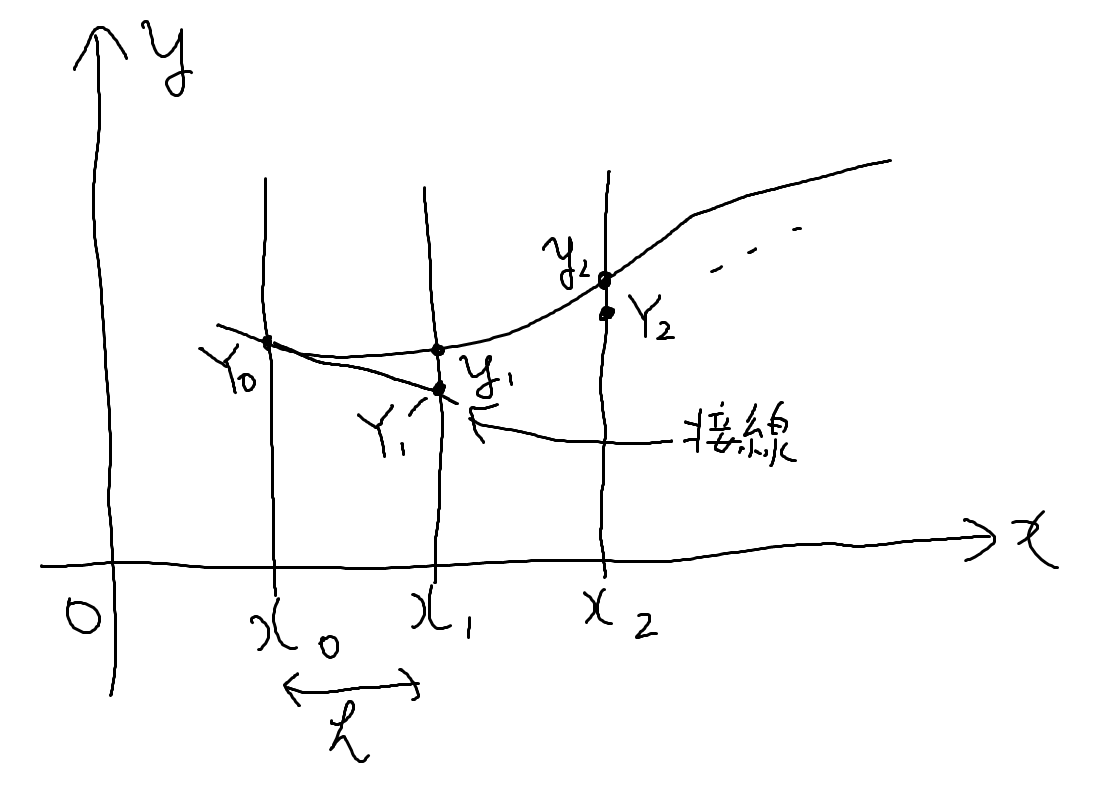
\includegraphics[width=7cm]{img/4-euler.png}
  \caption{オイラー法のイメージ}
  \label{fig:4-euler}
\end{figure}

図\ref{fig:4-euler}のように、$h$ごとに取られた各点$x_i$に対して、それぞれに対応する正しい$y$の値$y_i$、および計算機で計算した近似値$Y_i$を考えます。このとき、$h$を「刻み幅」と言います。刻み幅は一定である必要はありませんが、ここでは一定としておきます。

この考え方を使うと、$Y_{i+1}$は漸化式のように、

\begin{eqnarray}
    Y_{i+1}=Y_i+hf(x_i,Y_i)
\end{eqnarray}

\noindent
と書けます。この式を使って初期条件$x_0$で$Y_0$から順番に$x$を進めていくことで、関数$y$の近似を求めることができます。

擬似コードを以下に示します。

\begin{algorithm}
\caption{オイラー法}
\begin{algorithmic}
\REQUIRE $x_0,Y_0,h,N$
\ENSURE $Y_N$
\FOR{$i=0$ \TO $N-1$}
    \STATE $x_i\Leftarrow x_{i-1}+h$
    \STATE $Y_{i+1}\Leftarrow Y_i+hf(x_i,Y_i)$
\ENDFOR
\RETURN $Y_N$
\end{algorithmic}
\end{algorithm}

$h$の2乗以上の項を無視したので、局所誤差\footnote{一回の計算につき生じうる誤差のことです}は$O(h^2)$です。

また、誤差の蓄積を考えれば、最終的に得られる計算結果に含まれる誤差\footnote{計算を繰り返し、最終的に生じうる誤差のことです}は

\begin{eqnarray}
    O(h^2)\times \frac{x_N-x_0}{h}=O(h)
\end{eqnarray}

となり、$O(h)$の誤差が含まれていると言えます。







\section{改良オイラー法(中点法)}
\label{adv-euler}
オイラー法は計算が軽い反面、言ってしまえば精度がいまいちでした。そこで、簡単に精度を上げる方法として図\ref{fig:4-adv-euler}の方法を考えます。

\begin{figure}[ht!]
  \centering
  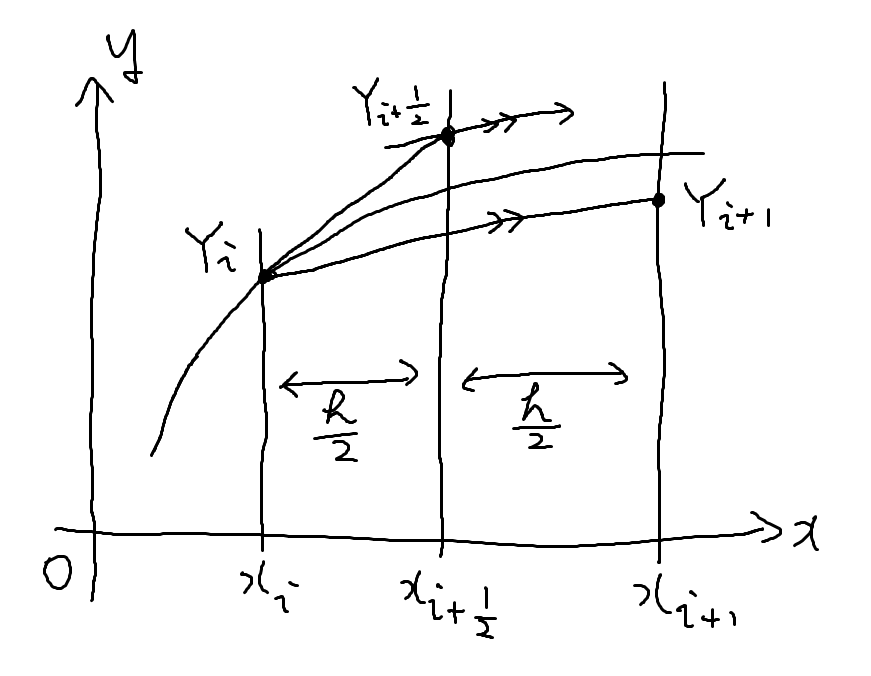
\includegraphics[width=10cm]{img/4-adv-euler.png}
  \caption{改良オイラー法のイメージ}
  \label{fig:4-adv-euler}
\end{figure}

これは、

\begin{enumerate}
    \item 通常のオイラー法を使って$Y_{i+1/2}$を求める
    \item 微分方程式から$Y_{i+1/2}$での勾配$k$を求める
    \item $Y_{i+1}=Y_i+hk$として$Y_{i+1}$を定める
\end{enumerate}

という手順を踏んでいます。改良オイラー法は勾配として点$Y_{i+1/2}$での傾きを使うことに特徴があります。これを擬似コードにすると以下になります。解く微分方程式はオイラー法と同じ式\ref{eq:differential-1}とします。

\begin{algorithm}
\caption{改良オイラー法}
\begin{algorithmic}
\REQUIRE $x_0,Y_0,h,N$
\ENSURE $Y_N$
\FOR{$i=0$ \TO $N-1$}
    \STATE $x_{i+1/2}\Leftarrow x_i+\frac{h}{2}$
    \STATE $Y_{i+1/2}\Leftarrow Y_i+\frac{h}{2}f(x_i,Y_i)$
    \STATE $Y_{i+1}\Leftarrow Y_i+hf(x_{i+1/2},Y_{i+1/2})$
\ENDFOR
\RETURN $Y_N$
\end{algorithmic}
\end{algorithm}

計算はオイラー法よりも多少重くなってしまいました(とは言っても定数倍です)が、精度はかなり良くなりました。実際に誤差を見積もってみましょう。改良オイラー法は、擬似コードを1つの式にすれば、

\begin{eqnarray}
    Y_{i+1}=Y_i+hf\pqty{x_{i+1/2},Y_i+\frac{h}{2}f(x_i,Y_i)}
\end{eqnarray}

\noindent
です。$f(x,y)=\dd y/\dd x$とオイラー法で出てきたテイラー展開式\ref{eq:taylor}を使って展開してみましょう。

\begin{eqnarray}
    Y_{i+1}&=&Y_i+h\pqty{\frac{\dd}{\dd x}y\pqty{x_i+\frac{h}{2}}} \\
    &=&Y_i+h\frac{\dd}{\dd x}\pqty{y(x_i)+\frac{h}{2}\frac{\dd}{\dd x}y(x_i)} \nonumber \\
    &=&Y_i+h\frac{\dd}{\dd x}y(x_i)+\frac{h^2}{2}\frac{\dd^2}{\dd x^2}y(x_i) \setcounter{equation}{9}
\end{eqnarray}

テイラー展開式\ref{eq:taylor}と比べると、3次の項まで一致しています。よって局所誤差は$O(h^3)$です。よって、最終的に生じうる誤差は

\begin{eqnarray}
    O(h^3)\times \frac{x_N-x_0}{h}=O(h^2)
\end{eqnarray}

です。オイラー法は$O(h)$でしたので、ぐんと誤差が小さくなりましたね。







\section{ルンゲ・クッタ法}
\label{runge-kutta}
ここではまず狭義のルンゲ・クッタ法を紹介し、その後に一般化されたルンゲ・クッタ法を紹介します。

オイラー法や改良オイラー法は

\begin{eqnarray}
    Y_{i+1}=Y_i+h\Phi(x_i,Y_i)
\end{eqnarray}

\noindent
という形の式をしていました。ルンゲ・クッタ法ではこの式について$\Phi$を工夫することで精度を高める試みをしています。オイラー法や改良オイラー法では勾配を1つだけ求め、それを採用していましたが、ルンゲ・クッタ法では勾配を複数求め、その重みつき平均を勾配とします。

狭義のルンゲ・クッタ法は、「4段4次のルンゲ・クッタ法」と呼ばれ、

\begin{eqnarray}
    k_1&=&f(x_i,Y_i) \\
    k_2&=&f\pqty{x_i+\frac{h}{2},Y_i+\frac{k_1}{2}} \\
    k_3&=&f\pqty{x_i+\frac{h}{2},Y_i+\frac{k_2}{2}} \\
    k_4&=&f(x_i+h,Y_i+hk_3)
\end{eqnarray}

\noindent
として勾配$k_1$から$k_4$を定義して、

\begin{eqnarray}
    Y_{i+1}=Y_i+\frac{h}{6}(k_1+2k_2+2k_3+k_4)
    \label{eq:runge-kutta}
\end{eqnarray}

\noindent
として$Y_{i+1}$を求めます。たくさん$k$が出てきましたが、これらは、

\clearpage

\begin{itemize}
    \item $k_1$は$x_i$での勾配(通常のオイラー法で使う勾配)
    \item $k_2$は$x_{i+1/2}$での勾配(改良オイラー法で使う勾配)
    \item $k_3$は$k_2$の値から推測した$Y_{i+1/2}$を使用した、$x_{i+1/2}$での勾配
    \item $k_4$は$k_3$の値から推測した$Y_{i+1}$を使用した、$x_{i+1}$での勾配
\end{itemize}

\noindent
という意味を持ちます。$k$を図にすると図\ref{fig:4-runge-kutta}となります。

\begin{figure}[ht!]
  \centering
  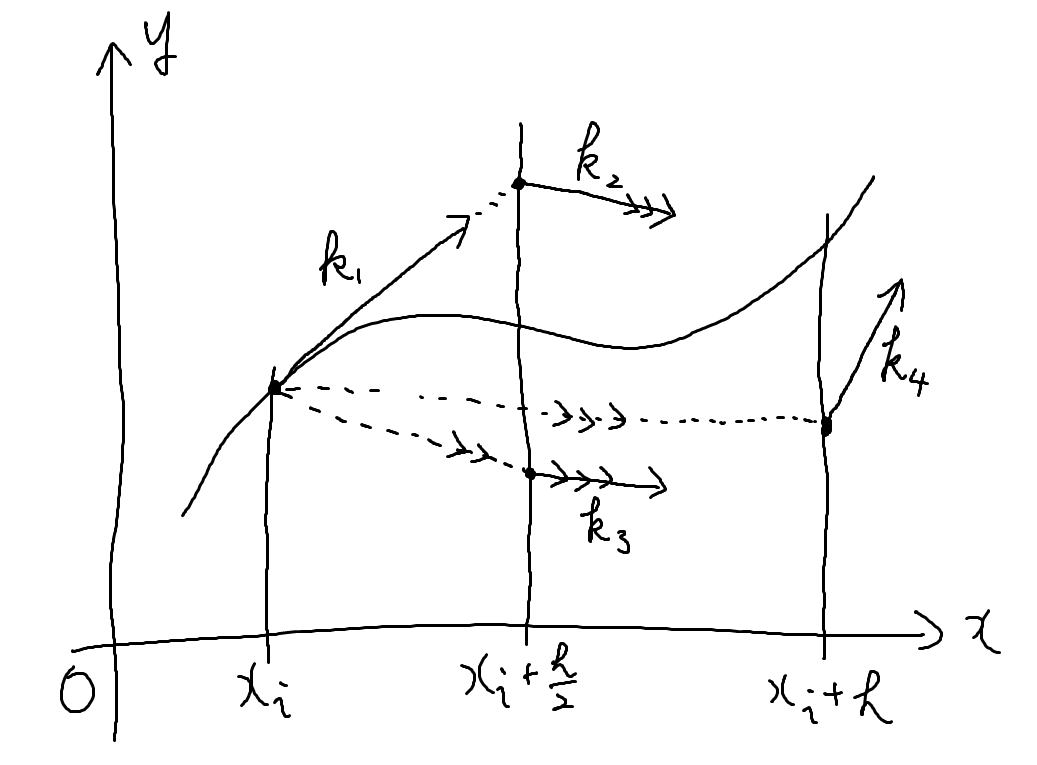
\includegraphics[width=10cm]{img/4-runge-kutta.png}
  \caption{4段4次ルンゲ・クッタ法のイメージ}
  \label{fig:4-runge-kutta}
\end{figure}

これらの$k$を重みをつけて平均し、$Y_{i+1}$を求めるときに使う勾配とします。

擬似コードにすると以下です。

\begin{algorithm}
\caption{4段4次ルンゲ・クッタ法}
\begin{algorithmic}
\REQUIRE $x_0,Y_0,h,N$
\ENSURE $Y_N$
\FOR{$i=0$ \TO $N-1$}
    \STATE $x_i\Leftarrow x_{i-1}+h$
    \STATE $k_1\Leftarrow f(x_i,Y_i)$
    \STATE $k_2\Leftarrow f\pqty{x_i+\frac{h}{2},Y_i+\frac{k_1}{2}}$
    \STATE $k_3\Leftarrow f\pqty{x_i+\frac{h}{2},Y_i+\frac{k_2}{2}}$
    \STATE $k_4\Leftarrow (x_i+h,Y_i+hk_3)$
    \STATE $Y_{i+1}\Leftarrow Y_i+\frac{h}{6}(k_1+2k_2+2k_3+k_4)$
\ENDFOR
\RETURN $Y_N$
\end{algorithmic}
\end{algorithm}

4段4次のルンゲ・クッタ法の誤差を見積もってみましょう。各$k$について$\dd y/\dd x$を使った形に書き換え、最後にルンゲ・クッタ法の式\ref{eq:runge-kutta}に代入します。

まずは$k_1$についてです。

\begin{eqnarray}
    k_1&=&\frac{\dd}{\dd x}y(x_i)
\end{eqnarray}

$k_2$については、

\begin{eqnarray}
    k_2&=&\frac{\dd}{\dd x}y\pqty{x_i+\frac{h}{2}} \\
    &=&\frac{\dd}{\dd x}\pqty{y(x_i)+\frac{h}{2}\frac{\dd}{\dd x}y(x_i)} \nonumber \\
    &=&\frac{\dd}{\dd x}y(x_i)+\frac{h}{2}\frac{\dd^2}{\dd x^2}y(x_i) \setcounter{equation}{19}
\end{eqnarray}

$k_3$は、

\begin{eqnarray}
    k_3&=&\frac{\dd}{\dd x}y\pqty{x_i+\frac{h}{2}} \\
    &=&\frac{\dd}{\dd x}\pqty{y(x_i)+\frac{h}{2}\frac{\dd}{\dd x}y\pqty{x_i+\frac{h}{2}}} \ \mbox{($k_2$の傾きを使う)} \nonumber \\
    &=&\frac{\dd}{\dd x}\pqty{y(x_i)+\frac{h}{2}\pqty{\frac{\dd}{\dd x}y(x_i)+\frac{h}{2}\frac{\dd^2}{\dd x^2}y(x_i)}} \nonumber \\
    &=&\frac{\dd}{\dd x}y(x_i)+\frac{h}{2}\frac{\dd^2}{\dd x^2}y(x_i)+\frac{h^2}{4}\frac{\dd^3}{\dd x^3}y(x_i) \setcounter{equation}{21}
\end{eqnarray}

最後に$k_4$です。

\begin{eqnarray}
    k_4&=&\frac{\dd}{\dd x}y(x_i+h) \\
    &=&\frac{\dd}{\dd x}\pqty{y(x_i)+h\frac{\dd}{\dd x}y\pqty{x_i+\frac{h}{2}}}\ \mbox{($k_3$の傾きを使う)} \nonumber \\
    &=&\frac{\dd}{\dd x}\pqty{y(x_i)+h\pqty{\frac{\dd}{\dd x}y(x_i)+\frac{h}{2}\frac{\dd^2}{\dd x^2}y(x_i)+\frac{h^2}{4}\frac{\dd^3}{\dd x^3}y(x_i)}} \nonumber \\
    &=&\frac{\dd}{\dd x}y(x_i)+h\frac{\dd^2}{\dd x^2}y(x)+\frac{h^2}{2}\frac{\dd^3}{\dd x^3}y(x_i)+\frac{h^3}{4}\frac{\dd^4}{\dd x^4}y(x_i) \setcounter{equation}{23}
\end{eqnarray}

さて、では4段4次のルンゲ・クッタ法の式\ref{eq:runge-kutta}に代入しましょう。

\begin{eqnarray}
    Y_{i+1}&=&Y_i+\frac{h}{6}\frac{\dd}{\dd x}y(x_i)
    +\frac{h}{3}\pqty{\frac{\dd}{\dd x}y(x_i)+\frac{h}{2}\frac{\dd^2}{\dd x^2}y(x_i)} \nonumber \\
    &+&\frac{h}{3}\pqty{\frac{\dd}{\dd x}y(x_i)+\frac{h}{2}\frac{\dd^2}{\dd x^2}y(x_i)+\frac{h^2}{4}\frac{\dd^3}{\dd x^3}y(x_i)} \nonumber \\
    &+&\frac{h}{6}\pqty{\frac{\dd}{\dd x}y(x_i)+h\frac{\dd^2}{\dd x^2}y(x)+\frac{h^2}{2}\frac{\dd^3}{\dd x^3}y(x_i)+\frac{h^3}{4}\frac{\dd^4}{\dd x^4}y(x_i)} \setcounter{equation}{24}\\
    &=&Y_i+h\frac{\dd}{\dd x}y(x_i)+\frac{h^2}{2}\frac{\dd^2}{\dd x^2}y(x_i)+\frac{h^3}{6}\frac{\dd^3}{\dd x^3}y(x_i)+\frac{h^4}{24}\frac{\dd^4}{\dd x^4}y(x_i) \setcounter{equation}{25}
\end{eqnarray}

綺麗にテイラー展開の式\ref{eq:taylor}と4次の項まで一致しました。よって、4段4次ルンゲ・クッタ法の局所誤差は$O(h^5)$、最終的に生じうる誤差は$O(h^4)$です。実は「4段」は$k$の数である4つ、「4次」は最終的な誤差の次数$O(h^4)$の4です。








\subsection{一般的なルンゲ・クッタ法}
\label{runge-kutta-general}
$n$段のルンゲ・クッタ法は、

\begin{eqnarray}
    k_i=f\pqty{x_i+hc,Y_i+h\sum_{j=1}^{i-1}a_{i\ j}k_j}
\end{eqnarray}

\noindent
として、

\begin{eqnarray}
    Y_{i+1}=Y_i+\sum_{i=1}^n b_i k_i
\end{eqnarray}

\noindent
と書けます。なお、$m$次の精度を出すために必要な最低段数は

\begin{table}[htb]
\begin{center}
  \caption{$m$次のルンゲ・クッタ法に必要な最低の次数$n$}
  \begin{tabular}{c|cccccccc}
    $m$次 & 1 & 2 & 3 & 4 & 5 & 6 & 7 & 8 \\
    \hline
    $n$段 & 1 & 2 & 3 & 4 & 6 & 7 & 9 & 11 \\
  \end{tabular}
  \end{center}
\end{table}

\noindent
です。

ちなみにオイラー法は「1段1次ルンゲ・クッタ法」、改良オイラー法は「2段2次ルンゲ・クッタ法」です。









\section{連立微分方程式}
\label{numerical-multiple}
これまでは一つの微分方程式を解いてきました、ここでは連立微分方程式を解きます。連立微分方程式は全て1階で\footnote{高階の微分方程式も連立微分方程式へと帰着できるため、実は構成する微分方程式は高階であっても良いのです。高階微分方程式は次節で扱います。}、$n$個あるとします。それぞれの微分方程式は

\begin{eqnarray}
    \frac{\dd y_i}{\dd x}=f_i(x,y_1,y_2,\dots,y_n)
\end{eqnarray}

\noindent
と表せるとします。すると、ベクトル

\begin{eqnarray}
    \boldsymbol{y}&=&(y_1,y_2,\dots,y_n) \\
    \boldsymbol{f}(x,\boldsymbol{y})&=&\pqty{
    \begin{array}{c}
        f_1(x,y_1,y_2,\dots,y_n) \\
        f_2(x,y_1,y_2,\dots,y_n) \\
        \vdots \\
        f_n(x,y_1,y_2,\dots,y_n)
    \end{array}
    }
\end{eqnarray}

\noindent
を使って、

\begin{eqnarray}
    \frac{\dd\boldsymbol{y}}{\dd x}=\boldsymbol{f}(x,\boldsymbol{y})
    \label{eq:numerical-multiple}
\end{eqnarray}

\noindent
というように微分方程式をすっきり表すことができます。このとき、初期条件を$x=x_0$で、

\begin{eqnarray}
    \boldsymbol{Y_0}=(y_{1\ 0},y_{2\ 0},\dots,y_{n\ 0})
\end{eqnarray}

\noindent
と定めます。

式\ref{eq:numerical-multiple}は一階の微分方程式\ref{eq:differential-1}が単にベクトルになったものではないでしょうか。というわけで、連立微分方程式も難しいことはありません。一階の微分方程式と同様に解くことができます。オイラー法を使った場合の擬似コードを以下に示します。

\begin{algorithm}
\label{al:multiple}
\caption{連立微分方程式でのオイラー法}
\begin{algorithmic}
\REQUIRE $x_0,\boldsymbol{Y_0},h,N$
\ENSURE $\boldsymbol{Y_N}$
\FOR{$i=0$ \TO $N-1$}
    \STATE $x_i\Leftarrow x_{i-1}+h$
    \FOR{$j=0$ \TO $n-1$}
        \STATE $\boldsymbol{Y_{i+1}}[j]\Leftarrow \boldsymbol{Y_i}[j]+h\boldsymbol{f}(x_i,\boldsymbol{Y_i})[j]$
    \ENDFOR
\ENDFOR
\RETURN $\boldsymbol{Y_N}$
\end{algorithmic}
\end{algorithm}








\section{高階微分方程式}
\label{higher}
高階微分方程式

\begin{eqnarray}
    \frac{\dd^ny}{\dd x^n}=f\pqty{x,y,\frac{\dd y}{\dd x},\frac{\dd^2 y}{\dd x^2},\dots,\frac{\dd^{n-1} y}{\dd x^{n-1}}}
\end{eqnarray}

\noindent
を考えましょう。また、初期条件を$x=x_0$において

\begin{eqnarray}
    y&=&y_{1\ 0} \nonumber \\
    \frac{\dd y}{\dd x}&=&y_{2\ 0} \nonumber \\
    \frac{\dd^2 y}{\dd x^2}&=&y_{3\ 0} \nonumber \\
    \vdots \nonumber \\
    \frac{\dd^{n-1} y}{\dd x^{n-1}}&=&y_{n\ 0} \setcounter{equation}{34}
\end{eqnarray}

\noindent
とします。ここで、見やすくするために

\begin{eqnarray}
    y&=&y_1 \nonumber \\
    \frac{\dd y}{\dd x}&=&y_2 \nonumber \\
    \frac{\dd^2 y}{\dd x^2}&=&y_3 \nonumber \\
    \vdots \nonumber \\
    \frac{\dd^{n-1} y}{\dd x^{n-1}}&=&y_n \setcounter{equation}{35}
\end{eqnarray}

\noindent
を導入すると、$y_i$同士の関係として全ての$i<n$について

\begin{eqnarray}
    \frac{\dd y_i}{\dd x}=y_{i+1}
    \label{eq:numerical_ys}
\end{eqnarray}

\noindent
が導かれ、元の微分方程式は

\begin{eqnarray}
    \frac{\dd y_n}{\dd x}=f(x,y_1,y_2,\dots,y_n)
    \label{eq:higher}
\end{eqnarray}

\noindent
と表せます。式\ref{eq:numerical_ys}と式\ref{eq:higher}を合わせるとなんと一階の連立微分方程式になってしまいました。これで\ref{numerical-multiple}節の方法で解くことができます。擬似コードはアルゴリズム\ref{al:multiple}とほぼ同じなので割愛します。








\section{予測子修正子法}
\label{numerical-integrate}
微分方程式\ref{eq:differential-1}を解くとして、$x_i$、$x_{i+1}$に対応する値$y_i$と$y_{i+1}$は

\begin{eqnarray}
    y_{i+1}-y_i=\int_{x_i}^{x_{i+1}}f(x,y)\dd x
    \label{eq:numerical-integrate}
\end{eqnarray}

\noindent
という関係を持っています。この右辺をどう精度よく近似するかが問題です。$x_i$に対応する$Y_i$がすでにわかっているとして、右辺の$f(x,y)$を$f(x_i,Y_i)$と近似すると、刻み幅を$h$として

\begin{eqnarray}
    Y_{i+1}=Y_i+hf(x_i,Y_i) \nonumber
\end{eqnarray}

\noindent
となります。これはまさにオイラー法です。

では次に式\ref{eq:numerical-integrate}の右辺にある積分を、台形公式\footnote{定積分を数値的に計算する手法の一つです。}

\begin{eqnarray}
    \int_{x_i}^{x_{i+1}}f(x,y)\dd x \fallingdotseq \frac{x_{i+1}-x_i}{2}(f(x_i,y_i)+f(x_{i+1},y_{i+1}) \setcounter{equation}{39}
\end{eqnarray}

\noindent
を使うと、

\begin{eqnarray}
    Y_{i+1}=Y_i+\frac{h}{2}(f(x_i,Y_i)+f(x_{i+1},Y_{i+1}))
    \label{eq:numerical-trapezoid}
\end{eqnarray}

\noindent
となります。ちょっと待って下さい。右辺に$Y_{i+1}$があります。このままでは計算できません。

このように、未知の値を求めるために未知の値を必要とする解法を「陰解法」と言います。対してこれまで解説してきたように、未知の値を求めるのに既知の値のみを必要とする解法を「陽解法」と言います。

陰解法は少し面倒ですが、以下の手順で解くことができます。

\begin{enumerate}
    \item $Y_{i+1}$の近似値$Y_{i+1}^{(0)}$を適当に決める。
    \item 式\ref{eq:numerical-trapezoid}の右辺の$Y_{i+1}$に$Y_{i+1}^{(j)}$を代入し、左辺$Y_{i+1}^{(j+1)}$を求める。
    \item 十分小さな正の値$\epsilon$を使って$|Y_{i+1}^{(j)}-Y_{i+1}^{(j+1)}|<\epsilon$となるまで2を繰り返す。
\end{enumerate}

最初に$Y_{i+1}^{(0)}$を決めるときにはオイラー法を使うのが良いでしょう。最初に$Y_{i+1}^{(0)}$を決める演算を「予測子」、その後に繰り返し式\ref{eq:numerical-trapezoid}を使って$Y_{i+1}^{(j)}$を更新する演算を「修正子」と言います。そしてこのように繰り返し演算して精度良く$Y_{i+1}$を求める手法を「予測子修正子法」と言います。

通常は修正子の反復回数が1回または2回となるくらいに刻み幅$h$を小さくします。

擬似コードはこちらです。

\begin{algorithm}
\label{al:predictor-Corrector}
\caption{予測子修正子法}
\begin{algorithmic}
\REQUIRE $x_0,Y_0,h,N,\epsilon$
\ENSURE $Y_N$
\FOR{$i=0$ \TO $N-1$}
    \STATE $x_i\Leftarrow x_{i-1}+h$
    \STATE $x_{i+1}\Leftarrow x_i+h$
    \WHILE{$|Y_{i+1}'-Y_{i+1}|\geq\epsilon$}
        \STATE $Y_{i+1}'\Leftarrow Y_{i+1}$
        \STATE $Y_{i+1}\Leftarrow Y_i+\frac{h}{2}(f(x_i,Y_i)+f(x_{i+1},Y_{i+1}'))$
    \ENDWHILE
\ENDFOR
\RETURN $Y_N$
\end{algorithmic}
\end{algorithm}










\section{差分法}
\label{difference}
ここまで解いてきた微分方程式は、ある初期値$x=x_0$で$y=Y_0$がわかっていて、そこから$x$を少しずつ進めていく方法を取っていました。これを初期値問題と言います。一方で、$x$の定義域の端での値が求まっている微分方程式が存在します。これが境界値問題です。本節ではこの境界値問題を扱います。

境界値問題の例として、二階の微分方程式

\begin{eqnarray}
    \frac{\dd^2 y}{\dd x^2}=f\pqty{x,y,\frac{\dd y}{\dd x}} \\
    y(x_0)=y_0,\ y(x_N)=y_N
\end{eqnarray}

を用いることにしましょう。ここで、$x_0,x_N$は定義域の端にあるとします。

境界値問題を解くために、まずは関数$y(x)$の導関数を近似的に表すことから始めましょう。微分の定義は

\begin{eqnarray}
    \frac{\dd}{\dd x}y(x)=\lim_{h\rightarrow0}\frac{y(x+h)-y(x)}{h}
\end{eqnarray}

\noindent
でした。計算機は極限を扱うことができないので、数値解析では微分をある有限の小さな値$h$を使って

\begin{eqnarray}
    \frac{\dd}{\dd x}y(x)=\frac{y(x+h)-y(x)}{h}
    \label{eq:advance}
\end{eqnarray}

\noindent
と表すことにします。ここで、導関数の導出をもう一つ考えてみましょう。

\begin{eqnarray}
    \frac{\dd}{\dd x}y(x)=\frac{y(x)-y(x-h)}{h}
    \label{eq:retreat}
\end{eqnarray}

\noindent
こちらも導関数の近似として使えないでしょうか。

これらの式にある$y(x+h)-y(x)$のような量を「差分」と言います。そして、式\ref{eq:advance}の差分を「前進差分」、式\ref{eq:retreat}の差分を「後退差分」と言います。このように差分を用いて導関数を近似することを「差分近似」と言います。特に式\ref{eq:advance}を「前進差分近似」、式\ref{eq:retreat}を「後退差分近似」と言います。

では前進差分近似の誤差を考えてみましょう。$y(x+h)$をテイラー展開すると、

\begin{eqnarray}
    \label{eq:advance-taylor}
    y(x+h)=y(x)+h\frac{\dd}{\dd x}y(x)+\frac{h^2}{2!}\frac{\dd^2}{\dd x^2}y(x)+\frac{h^3}{3!}\frac{\dd^3}{\dd x^3}y(x)+\dots
\end{eqnarray}

\noindent
となります。この式を変形すると、

\begin{eqnarray}
    \frac{y(x+h)-y(x)}{h}=\frac{\dd}{\dd x}y(x)+\frac{h}{2!}\frac{\dd^2}{\dd x^2}y(x)+\dots
\end{eqnarray}

\noindent
となり、式\ref{eq:advance}と比べると誤差が$O(h)$だとわかります。

後退差分近似についても同じように考えると、

\begin{eqnarray}
    \label{eq:retreat-taylor}
    y(x-h)&=&y(x)-h\frac{\dd}{\dd x}y(x)+\frac{h^2}{2!}\frac{\dd^2}{\dd x^2}y(x)-\frac{h^3}{3!}\frac{\dd^3}{\dd x^3}y(x)+\dots \\
    \frac{y(x)-y(x-h)}{h}&=&\frac{\dd}{\dd x}y(x)-\frac{h}{2!}\frac{\dd^2}{\dd x^2}y(x)+\dots
\end{eqnarray}

\noindent
となり、前進差分近似と同じく誤差は$O(h)$です。

前進差分近似と後退差分近似よりも誤差の少ない方法を考えましょう。式\ref{eq:advance-taylor}と式\ref{eq:retreat-taylor}を辺々引くと、

\begin{eqnarray}
    y(x+h)-y(x-h)&=&2h\frac{\dd}{\dd x}y(x)+2\frac{h^3}{3!}\frac{\dd^3}{\dd x^3}y(x)+\dots \\
    \frac{y(x+h)-y(x-h)}{2h}&=&\frac{\dd}{\dd x}y(x)+\frac{h^2}{3!}\frac{\dd^3}{\dd x^3}y(x)+\dots
\end{eqnarray}

\noindent
となり、別の近似を考えられます。この左辺を$\dd y(x)/\dd x$の近似として用いれば、誤差は$O(h^2)$となり、前進差分近似、後退差分近似よりも精度の良い近似となりました。これを「中心差分近似」と言います。

前進差分近似、後退差分近似、中心差分近似をまとめて図にすると図\ref{fig:4-difference}になります。

なお、$y(x+2h),y(x+h),y(x-h),y(x-2h)$のテイラー展開も使って作った中心差分近似を4次中心差分近似と言います。この差分近似も時々紹介されます。

\begin{figure}[ht!]
  \centering
  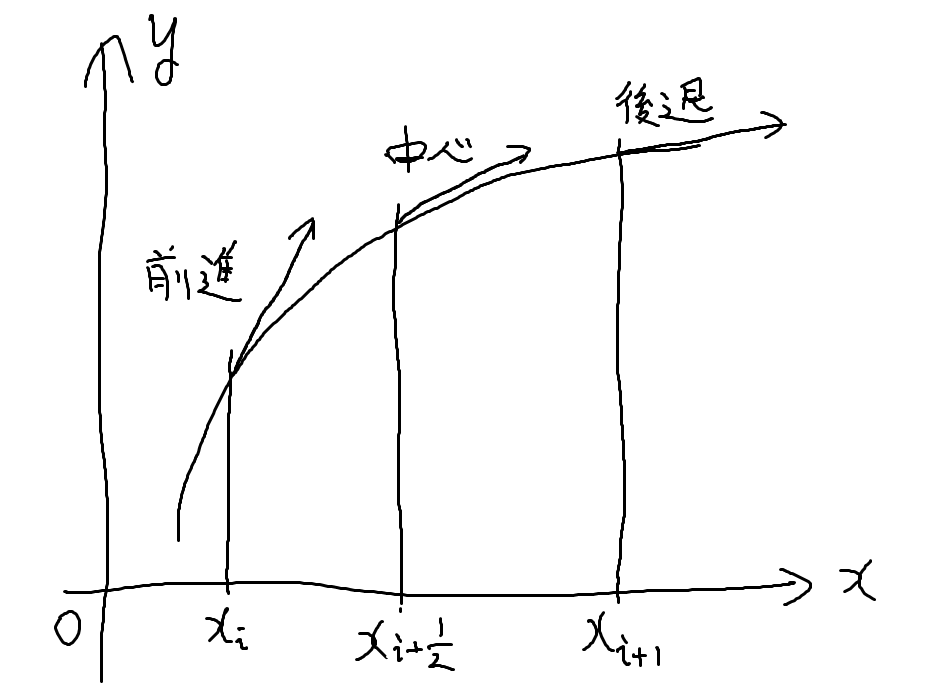
\includegraphics[width=10cm]{img/4-difference.png}
  \caption{差分近似のイメージ}
  \label{fig:4-difference}
\end{figure}

次に二階の導関数を考えましょう。式\ref{eq:advance-taylor}と式\ref{eq:retreat-taylor}を辺々足すと、

\begin{eqnarray}
    y(x+h)+y(x-h)&=&2y(x)+2\frac{h^2}{2!}\frac{\dd^2}{\dd x^2}y(x)+2\frac{h^4}{4!}\frac{\dd^4}{\dd x^4}y(x)+\dots \\
    \frac{y(x+h)-2y(x)+y(x-h)}{h^2}&=&\frac{\dd^2}{\dd x^2}y(x)+2\frac{h^2}{4!}\frac{\dd^4}{\dd x^4}y(x)
\end{eqnarray}

\noindent
となり、誤差が$O(h^2)$の二階導関数ができました。これは「二階導関数の中心差分近似」と言います。

では微分方程式を解きましょう。微分方程式を$x_i,Y_{i-1}Y_i,Y_{i+1}$を使って書き直すと、これまでの近似から、

\begin{eqnarray}
    \frac{Y_{i+1}-2Y_i+Y_{i-1}}{h^2}=f\pqty{x_i,Y_i,\frac{Y_{i+1}-Y_{i-1}}{2h}}
    \label{eq:difference-original}
\end{eqnarray}

\noindent
となります。このように、差分近似を用いて導いた式を「差分方程式」と言います。また、その解を「差分解」と言います。

少し具体的な方程式として二階線形微分方程式

\begin{eqnarray}
    \frac{\dd^2 y}{\dd x^2}=P(x)\frac{\dd y}{\dd x}+Q(x)y+R(x)
\end{eqnarray}

\noindent
を考えてみましょう。ここで、$P(x)$、$Q(x)$、$R(x)$は既知の関数です。この問題を式\ref{eq:difference-original}を使って書き直すと、

\begin{eqnarray}
    \frac{Y_{i+1}-2Y_i+Y_{i-1}}{h^2}=P(x_i)\frac{Y_{i+1}-Y_{i-1}}{2h}+Q(x_i)Y_i+R(x_i)
\end{eqnarray}

\noindent
となります。これを整理して、

\begin{eqnarray}
    \pqty{1-\frac{1}{2}hP(x_i)}Y_{i+1}-(2+h^2Q(x_i))Y_i+\pqty{1+\frac{1}{2}hP(x_i)}Y_{i-1}=h^2R(x_i)
\end{eqnarray}

\noindent
を得ます。これを、

\begin{eqnarray}
    a_i&=&1+\frac{1}{2}hP(x_i) \\
    b_i&=&-(2+h^2Q(x_i)) \\
    c_i&=&1-\frac{1}{2}hP(x_i)
\end{eqnarray}

\noindent
と置いて、

\begin{eqnarray}
    c_iY_{i+1}+b_iY_i+a_iY_{i-1}=h^2R(x_i)
\end{eqnarray}

\noindent
と書き換えます。この式を$i=1$から$i=N-1$まで並べて書いてみましょう。

\begin{eqnarray}
    \pqty{\begin{array}{ccccc}
        b_1 & c_1 & 0 & 0 & \hdots \\
        a_2 & b_2 & c_2 & 0 & \hdots \\
        0 & a_3 & b_3 & c_3 & \hdots \\
        \vdots & \vdots & \vdots & \vdots & \vdots \\
        \hdots & 0 & a_{N-2} & b_{N-2} & c_{N-2} \\
        \hdots & 0 & 0 & a_{N-1} & b_{N-1}
    \end{array}}
    \pqty{\begin{array}{c}
        Y_1 \\
        Y_2 \\
        Y_3 \\
        \vdots \\
        Y_{N-2} \\
        Y_{N-1}
    \end{array}}
    =\pqty{\begin{array}{c}
        h^2R(x_1)-a_1y_0 \\
        h^2R(x_2) \\
        h^2R(x_3) \\
        \vdots \\
        h^2R(x_{N-2}) \\
        h^2R(x_{N-1})-c_{N-1}y_N
    \end{array}}
    \label{eq:difference-liner-final}
\end{eqnarray}

一番上と一番下の行はそれぞれ定義域の境界なので、境界値を使って

\begin{eqnarray}
    c_1Y_2+b_1Y_1&=&h^2R(x_1)-a_1y_0 \\
    b_{N-1}Y_{N-1}+a_{N-1}Y_{N-2}&=&h^2R(x_{N-1})-c_{N-1}Y_N
\end{eqnarray}

\noindent
の式を用います。

これは単なる連立一次方程式ですね。ここで連立一次方程式の解き方を考えてみましょう。連立一次方程式の数値的な解き方には様々なものがありますが、ここでは式\ref{eq:difference-liner-final}に現れる行列が疎である\footnote{0が多いという意味です}性質を利用して効率的に解く方法(反復法)を2つ紹介します。







\subsubsection{ヤコビ法}
\label{jacobian}
式\ref{eq:difference-liner-final}の行列は常に対角成分($b_i$)が0でないとしましょう。すると、$a_i$を含む項と$c_i$を含む項を右辺に移項して、

\begin{eqnarray}
    \pqty{\begin{array}{ccccc}
        b_1 & 0 & 0 & 0 & \hdots \\
        0 & b_2 & 0 & 0 & \hdots \\
        0 & 0 & b_3 & 0 & \hdots \\
        \vdots & \vdots & \vdots & \vdots & \vdots \\
        \hdots & 0 & 0 & b_{N-2} & 0 \\
        \hdots & 0 & 0 & 0 & b_{N-1}
    \end{array}}
    \pqty{\begin{array}{c}
        Y_1 \\
        Y_2 \\
        Y_3 \\
        \vdots \\
        Y_{N-2} \\
        Y_{N-1}
    \end{array}}
    =\pqty{\begin{array}{c}
        h^2R(x_1)-a_1y_0-c_1Y_2 \\
        h^2R(x_2)-a_2Y_1-c_2Y_3 \\
        h^2R(x_3)-a_3Y_2-c_3Y_4 \\
        \vdots \\
        h^2R(x_{N-2})-a_{N-2}Y_{N-3}-c_{N-2}Y_{N-1} \\
        h^2R(x_{N-1})-a_{N-1}Y_{N-2}-c_{N-1}y_N
    \end{array}}
\end{eqnarray}

\noindent
と書き直すことができます。この中から1つ式を取り出すと、

\begin{eqnarray}
    b_nY_n=h^2R(x_n)-a_nY_{n-1}-c_nY_{n+1}
\end{eqnarray}

\noindent
という式になります。これを、

\begin{eqnarray}
    b_iY_i^{(j+1)}=h^2R(x_i)-a_iY_{i-1}^{(j)}-c_iY_{i+1}^{(j)}
\end{eqnarray}

\noindent
と読みかえるとどうでしょう。右辺は$j$回目に計算した$Y$の値、左辺は$j+1$回目に計算した$Y$の値になります。初期値$Y_1^{(0)}$から$Y_{N-1}^{(0)}$を適当に(全部0でOKです)設定してこの式を使って反復的に計算し、十分小さい正の$\epsilon$をによって$|Y_i^{(j)}-Y_i^{(j+1)}|<\epsilon$となったら計算を打ち切りましょう。

このようにして連立一次方程式を数値的に解くことができます。擬似コードを示します。

\begin{algorithm}
\label{al:difference-jacobian}
\caption{差分法(ヤコビ法を使用)}
\begin{algorithmic}
\REQUIRE $x_0,Y_0,Y_N,h,N,\epsilon$
\ENSURE $\boldsymbol{Y}$
\FOR{$i=1$ \TO $N-1$}
    \STATE $\boldsymbol{x}_i\Leftarrow x_{i-1}+h$
    \STATE $\boldsymbol{a}_i\Leftarrow 1+\frac{1}{2}hP(x_i)$
    \STATE $\boldsymbol{b}_i\Leftarrow -(2+h^2Q(x_i))$
    \STATE $\boldsymbol{c}_i\Leftarrow 1-\frac{1}{2}hP(x_i)$
\ENDFOR
\WHILE{at least one $|Y_{i+1}''-Y_{i+1}|\geq\epsilon$}
    \FOR{$i=1$ \TO $N-1$}
        \STATE $Y_i'\Leftarrow Y_i$
        \STATE $Y_i\Leftarrow h^2R(x_i)-\boldsymbol{a}_iY_{i-1}''-\boldsymbol{c}_iY_{i+1}''$
    \ENDFOR
\ENDWHILE
\FOR{$i=1$ \TO $N-1$}
    \STATE $Y_i''=Y_i'$
\ENDFOR
\RETURN $\boldsymbol{Y}$
\end{algorithmic}
\end{algorithm}








\subsubsection{ガウス・ザイデル法}
\label{gauss-seidel}
ヤコビ法の収束を早めた方法として、ガウス・ザイデル法があります。ヤコビ法では$Y_i^{(j+1)}$の値を求めるのに$Y_{i+1}^{(j)}$と$Y_{i-1}^{(j)}$の値を使っていましたが、ここで少し考えてみましょう。アルゴリズム\ref{al:difference-jacobian}を見ると、$Y_i^{(j+1)}$を求める時点で$Y_{i-1}^{(j+1)}$が求まっています。$Y_{i-1}^{(j)}$よりも$Y_{i-1}^{(j+1)}$を使った方が収束が早くなります。このように、$j+1$回目の計算をするときになるべく$j+1$回目にすでに行った計算結果を使う手法をガウス・ザイデル法と言います。これを擬似コードにするとヤコビ法より簡潔になります。

\begin{algorithm}
\label{al:difference-gauss-seidel}
\caption{差分法(ガウス・ザイデル法を使用)}
\begin{algorithmic}
\REQUIRE $x_0,Y_0,Y_N,h,N,\epsilon$
\ENSURE $\boldsymbol{Y}$
\FOR{$i=1$ \TO $N-1$}
    \STATE $\boldsymbol{x}_i\Leftarrow x_{i-1}+h$
    \STATE $\boldsymbol{a}_i\Leftarrow 1+\frac{1}{2}hP(x_i)$
    \STATE $\boldsymbol{b}_i\Leftarrow -(2+h^2Q(x_i))$
    \STATE $\boldsymbol{c}_i\Leftarrow 1-\frac{1}{2}hP(x_i)$
\ENDFOR
\WHILE{at least one $|Y_{i+1}'-Y_{i+1}|\geq\epsilon$}
    \FOR{$i=1$ \TO $N-1$}
        \STATE $Y_i'\Leftarrow Y_i$
        \STATE $Y_i\Leftarrow h^2R(x_i)-\boldsymbol{a}_iY_{i-1}'-\boldsymbol{c}_iY_{i+1}'$
    \ENDFOR
\ENDWHILE
\RETURN $\boldsymbol{Y}$
\end{algorithmic}
\end{algorithm}










\clearpage
%\chapter{数値的に偏微分方程式を解く}
\label{numerical-partial}
第\ref{analytical-partial}章でも少しお話ししましたが、偏微分方程式は複雑です。数値的に解くとしても統一的な方法はありません。ですので、ここでは基本的な偏微分方程式の形に絞ってその解き方を紹介します。

\section{問題設定}
\label{partial-problem}
ここでは基本的な偏微分方程式として、関数$u(x,y)$について、

\begin{eqnarray}
    A\frac{\partial^2u}{\partial x^2}+2B\frac{\partial^2u}{\partial x\partial y}+C\frac{\partial^2u}{\partial y^2}+D\frac{\partial u}{\partial x}+E\frac{\partial u}{\partial y}+Fu=f(x,y)
    \label{eq:partial-basic}
\end{eqnarray}

\noindent
を考えます。ここで、$A,B,C,D,E,F$は定数、$f(x,y)$は既知の関数だとします。

この形をした偏微分方程式は$AC-B^2$の値で分類でき、それぞれ

\begin{itemize}
    \item $AC-B^2>0$のとき「楕円型」
    \item $AC-B^2=0$のとき「放物型」
    \item $AC-B^2<0$のとき「双曲型」
\end{itemize}

\noindent
と言います。この型が違うと解$u$の挙動が大きく変わります。







\section{差分近似}
\label{partial-difference-calc}
常微分方程式の場合と同様に、2変数関数$u$の差分近似を考えます。まずは$u(x+h,y)$と$u(x-h,y)$についてテイラー展開します。

\begin{eqnarray}
    \label{eq:partial-u-x-1}
    u(x+h,y)&=&u(x,y)+h\frac{\partial}{\partial x}u(x,y)+\frac{h^2}{2!}\frac{\partial^2}{\partial x^2}u(x,y)+\frac{h^3}{3!}\frac{\partial^3}{\partial x^3}u(x,y)+\cdots \\
    \label{eq:partial-u-x-2}
    u(x-h,y)&=&u(x,y)-h\frac{\partial}{\partial x}u(x,y)+\frac{h^2}{2!}\frac{\partial^2}{\partial x^2}u(x,y)-\frac{h^3}{3!}\frac{\partial^3}{\partial x^3}u(x,y)+\cdots
\end{eqnarray}

準備は完了です。まずは$\partial u(x,y)/\partial x$の前進差分近似を求めます。\ref{euler-numerical}節の式を書き直すと、

\begin{eqnarray}
    \frac{\partial}{\partial x}u(x,y)&=&\frac{u(x+h,y)-u(x,y)}{h}+O(h)
\end{eqnarray}

\noindent
となります。これは式\ref{eq:partial-u-x-1}を移項した形をしています。同様にして$y$に関する微分は、

\begin{eqnarray}
    \frac{\partial}{\partial y}u(x,y)&=&\frac{u(x,y+k)-u(x,y)}{k}+O(k)
\end{eqnarray}

\noindent
です。

\if0
後の議論のために中心差分近似も求めておきましょう。式\ref{eq:partial-u-x-1}と式\ref{eq:partial-u-x-2}を辺々引くと、

\begin{eqnarray}
    u(x+h,y)-u(x-h,y)&=&2h\frac{\partial}{\partial x}u(x,y)+O(h^3) \\
    \frac{\partial}{\partial x}u(x,y)&=&\frac{u(x+h,y)-u(x-h,y)}{2h}+O(h^2)
\end{eqnarray}

\noindent
で、局所誤差は$O(h^2)$です。$y$についての微分も同様に、

\begin{eqnarray}
    \frac{\partial}{\partial y}u(x,y)&=&\frac{u(x,y+k)-u(x,y-k)}{2k}+O(k^2)
\end{eqnarray}

\noindent
です。
\fi

また、式\ref{eq:partial-u-x-1}と式\ref{eq:partial-u-x-2}を辺々足すと、

\begin{eqnarray}
    u(x+h,y)+u(x-h,y)&=&2u(x,y)+2\frac{h^2}{2!}\frac{\partial^2}{\partial x^2}u(x,y)+2\frac{h^4}{4!}\frac{\partial^4}{\partial x^4}u(x,y)+\cdots \\
    \frac{\partial^2}{\partial x^2}u(x,y)&=&\frac{u(x+h,y)-2u(x,y)+u(x-h,y)}{h^2}+O(h^2)
\end{eqnarray}

\noindent
二階微分の局所誤差は$O(h^2)$です。$y$についての微分も同様に、

\begin{eqnarray}
    \frac{\partial^2}{\partial y^2}u(x,y)&=&\frac{u(x,y+k)-2u(x,y)+u(x,y-k)}{k^2}+O(k^2)
\end{eqnarray}

最後に$u(x+h,y+k)$をテイラー展開して$\partial^2 u/(\partial x \partial y)$を求めましょう。

\begin{eqnarray}
    u(x+h,y+k)&=&u(x,y)+h\frac{\partial}{\partial x}u(x,y)+k\frac{\partial}{\partial y}u(x,y) \nonumber \\
    &+&\frac{h^2}{2!}\frac{\partial^2}{\partial x^2}u(x,y)+\frac{hk}{2!}2\frac{\partial^2}{\partial x\partial y}u(x,y)+\frac{k^2}{2!}\frac{\partial^2}{\partial y^2}u(x,y)+\cdots \setcounter{equation}{10}
\end{eqnarray}

\noindent
$u(x+h,y+k)$から$u(x+h,y),u(x,y+k)$をそれぞれ引いて、

\begin{eqnarray}
    u(x+h,y+k)-u(x+h,y)-u(x,y+k)=-u(x,y)+hk\frac{\partial^2}{\partial x\partial y}u(x,y)+O(hk(h+k))) \\
    \frac{\partial^2}{\partial x\partial y}u(x,y)=\frac{u(x+h,y+h)-u(x+h,y)-u(x,y+h)+u(x,y)}{hk}+O(hk(h+k)))
\end{eqnarray}

\noindent
とすることで目的の偏導関数が求まりました。局所誤差は$O(hk(h+k)))$です。








\section{陽的差分法}
\label{partial-difference-explicit}
実際に式\ref{eq:partial-basic}に\ref{partial-difference-calc}節での偏導関数を代入し、$u(x,y)=U_{i\ j},\ u(x+h,y)=U_{i+1\ j},\ u(x,y+k)=U_{i\ j+1},\ u(x+h,y+k)=U_{i+1\ j+1}$と置き、係数を適宜置いて、

\begin{eqnarray}
    \label{eq:partial-difference-former}
    2BhkU_{i+1\ j+1}+(Ak^2-2Bhk+Dhk^2)U_{i+1\ j}+(Ch^2-2Bhk+Eh^2k)U_{i\ j+1} \nonumber \\
    +(-2Ak^2+2Bhk-2Ch^2-Dhk^2-Eh^2k+h^2k^2F)U_{i\ j} \nonumber \\
    +Ak^2U_{i-1\ j}+Ch^2U_{i\ j-1}=h^2k^2f(x_i,y_j) \setcounter{equation}{13} \\
    \alpha U_{i+1\ j+1}+\beta U_{i+1\ j}+\gamma U_{i\ j+1}+\delta U_{i\ j}+\epsilon U_{i-1\ j}+\zeta U_{i\ j-1}=\eta f(x_i,y_j)
    \label{eq:partial-difference}
\end{eqnarray}

\noindent
としておきましょう。これを行列を使った式として書いてみます。空白は0です。

\begin{eqnarray}
    \pqty{\begin{array}{ccccc:ccccc:ccccc:c:ccc}
        \delta & \beta & & & & \gamma & \alpha & & & & & & & & & \cdots & & & \\
        \epsilon & \delta & \beta & & & & \gamma & \alpha & & & & & & & & \cdots & & & \\
        & \epsilon & \delta & \beta & & & & \gamma & \alpha & & & & & & & \cdots & & & \\
        & & \ddots & \ddots & \ddots & & & & \ddots & \ddots & & & & & & \cdots & & & \\ %[-2.5pt]
        & & & \epsilon & \delta & & & & & \gamma & & & & & & \cdots & & & \\
        \hdashline
        \zeta & & & & & \delta & \beta & & & & \gamma & \alpha & & & & \cdots & & & \\
        & \zeta & & & & \epsilon & \delta & \beta & & & & \gamma & \alpha & & & \cdots & & & \\
        & & \zeta & & & & \epsilon & \delta & \beta & & & & \gamma & \alpha & & \cdots & & & \\
        & & & \ddots & & & & \ddots & \ddots & \ddots & & & & \ddots & \ddots & \cdots & & & \\ %[-2.5pt]
        & & & & \zeta & & & & \epsilon & \delta & & & & & \gamma & \cdots & & & \\
        \hdashline
        & & & & & \zeta & & & & & \delta & \beta & & & & \cdots & & & \\
        & & & & & & \zeta & & & & \epsilon & \delta & \beta & & & \cdots & & & \\
        & & & & & & & \zeta & & & & \epsilon & \delta & \beta & & \cdots & & & \\
        & & & & & & & & \ddots & & & & \ddots & \ddots & \ddots & \cdots & & & \\
        & & & & & & & & & \zeta & & & & \epsilon & \delta & \cdots & & & \\
        \hdashline
        \vdots & \vdots & \vdots & \vdots & \vdots & \vdots & \vdots & \vdots & \vdots & \vdots & \vdots & \vdots & \vdots & \vdots & \vdots & \ddots & \vdots & \vdots & \vdots \\
        \hdashline
        & & & & & & & & & & & & & & & \cdots & \delta & & \\
        & & & & & & & & & & & & & & & \cdots & & \ddots & \\
        & & & & & & & & & & & & & & & \cdots & & & \delta \\
    \end{array}} \nonumber \\
    \pqty{\begin{array}{c}
        U_{1\ 1} \\
        U_{2\ 1} \\
        U_{3\ 1} \\
        \vdots \\
        U_{N-1\ 1} \\
        \hdashline
        U_{1\ 2} \\
        U_{2\ 2} \\
        U_{3\ 2} \\
        \vdots \\
        U_{N-1\ 2} \\
        \hdashline
        U_{1\ 3} \\
        U_{2\ 3} \\
        U_{3\ 3} \\
        \vdots \\
        U_{N-1\ 3} \\
        \hdashline
        \vdots \\
        \hdashline
        U_{1\ N-1} \\
        \vdots \\
        U_{N-1\ N-1}
    \end{array}}
    =\pqty{\begin{array}{c}
        \eta f(x_1,y_1)-\epsilon U_{0\ 1}-\zeta U_{1\ 0} \\
        \eta f(x_2,y_1)-\zeta U_{2\ 0} \\
        \eta f(x_3,y_1)-\zeta U_{3\ 0} \\
        \vdots \\
        \eta f(x_{N-1},y_1)-\alpha U_{N\ 2}-\beta U_{N\ 1}-\zeta U_{N-1\ 0} \\
        \hdashline
        \eta f(x_1,y_2)-\epsilon U_{0\ 2} \\
        \eta f(x_2,y_2) \\
        \eta f(x_3,y_2) \\
        \vdots \\
        \eta f(x_{N-1},y_2)-\alpha U_{N\ 3}-\beta U_{N\ 2} \\
        \hdashline
        \eta f(x_1,y_3)-\epsilon U_{0\ 3} \\
        \eta f(x_2,y_3) \\
        \eta f(x_3,y_3) \\
        \vdots \\
        \eta f(x_{N-1},y_3)-\alpha U_{N\ 4}-\beta U_{N\ 3} \\
        \hdashline
        \vdots \\
        \hdashline
        \eta f(x_1,y_{N-1})-\alpha U_{N\ N}-\gamma U_{N-1\ N} \\
        \vdots \\
        \eta f(x_{N-1},y_{N-1})-\alpha U_{N\ N}-\beta U_{N\ N-1}-\gamma U_{N-1\ N}
    \end{array}}
    \label{eq:numerical-partial-all}
    \setcounter{equation}{15}
\end{eqnarray}

ここで、境界条件として$(U_{0\ 0},U_{0\ 1}\cdots U_{0\ N})$、$(U_{1\ 0},U_{2\ 0}\cdots U_{N\ 0})$、$(U_{N\ 1},U_{N\ 2}\cdots U_{N\ N})$、\\\noindent$(U_{1\ N},U_{2\ N}\cdots U_{N-1\ N})$がわかっているとします。

陽的差分法の場合、$\alpha=0$である必要があります(そうでない場合は\ref{partial-difference-implicit}節でお話しします)。これは一見、巨大な連立一次方程式です。しかし、式\ref{eq:partial-difference}を見ると未知の量が$U_{i+1\ j}$、$X$を任意として既知の量が$U_{i\ X}$です。未知の量が一つしかないため、連立一次方程式ではなく個々の一次方程式を$i$が小さいものから順番に解くだけで済みます。

では実際に後の議論のため、拡散方程式

\begin{eqnarray}
    \frac{\partial u}{\partial t}=\frac{\partial^2u}{\partial x^2}
\end{eqnarray}

\noindent
を陽的差分法で解いてみましょう。問題にする領域は$0<x<1$かつ$0<t$とします。初期条件

\begin{eqnarray}
    t=0\mbox{で}u=\phi(x)
\end{eqnarray}

\noindent
および、境界条件

\begin{eqnarray}
    x=0,1\mbox{で}u=0
\end{eqnarray}

\noindent
が与えられているとします。

式\ref{eq:partial-basic}において、拡散方程式は$C=1, D=-1$($t$には$x,h$、$x$には$y,k$を対応させます)とし、残りを0とした方程式と見ることができます。よって、これは式\ref{eq:partial-difference}において、$\beta=-hk^2,\gamma=h^2,\delta=-2h^2+hk^2,\zeta=h^2$とし、残りを0とした方程式です。式\ref{eq:partial-difference}を書き直すと、

\begin{eqnarray}
    -hk^2U_{i+1\ j}+h^2U_{i\ j+1}+(-2h^2+hk^2)U_{i\ j}+h^2U_{i\ j-1}=0
\end{eqnarray}

\noindent
となります。これを整理して、

\begin{eqnarray}
    U_{i+1\ j}-U_{i\ j}=\frac{h}{k^2}(U_{i\ j+1}-2U_{i\ j}+U_{i\ j-1}) \\
    U_{i+1\ j}=\frac{h}{k^2}U_{i\ j+1}+\pqty{1-2\frac{h}{k^2}}U_{i\ j}+\frac{h}{k^2}U_{i\ j-1}
    \label{eq:diffusion}
\end{eqnarray}

\noindent
として、未知の$U_{i+1\ j}$を既知の$U_{i,X}$($X$は任意)のみで表せました。初期条件$U_{0\ X}$、および境界条件$U_{X\ 0},U_{X\ N}$($kN=1$)は既知なので、これで初期条件と境界条件を使ってこの偏微分方程式が数値的に解けます。

陽的差分法は$h$と$k$の条件によってはどれだけ$h$や$k$を小さくしても、解が厳密解から大きく外れることがあります。実際に陽的差分法で一つ偏微分方程式を解いてみて、この「解の安定性」を議論しましょう。











\subsection{フォン・ノイマンの安定性解析}
\label{explicit-stability}
陽的差分法で解いた拡散方程式の解の安定性を確かめましょう。ここでは、「フォン・ノイマンの安定性解析」を用います。まず関数$U(t_i,x)$が$x$の区間$(0,1)$でフーリエ級数展開可能だとしましょう\footnote{偏微分方程式を扱うときは大抵フーリエ級数展開可能ですが、もし不可能な場合には式\ref{eq:numerical-partial-all}の固有値の収束性を議論します。}。

関数$U_{i\ j}$を、$\mathrm{i}$を虚数単位、$C_{l\ i}$を未知定数として、

\begin{eqnarray}
    U_{i\ j}=\sum_{l=-\infty}^\infty C_{l\ i}e^{\mathrm{i}2\pi lx_j}
\end{eqnarray}

\noindent
と書くことにします。これを\ref{eq:diffusion}に代入し、$0<x_j<1$なので$x_j=jk$と置きます。すると$\sum$を外すことができ、それぞれの$l$について、

\begin{eqnarray}
    C_{l\ i+1}e^{\mathrm{i}2\pi ljk}&=&\frac{h}{k^2}C_{l\ i}e^{\mathrm{i}2\pi l(j+1)k}+\pqty{1-2\frac{h}{k^2}}C_{l\ i}e^{\mathrm{i}2\pi ljk}+\frac{h}{k^2}C_{l\ i}e^{\mathrm{i}2\pi l(j-1)k} \\
    C_{l\ i+1}&=&\pqty{\frac{h}{k^2}e^{\mathrm{i}2\pi lk}+1-2\frac{h}{k^2}+\frac{h}{k^2}e^{-\mathrm{i}2\pi lk}}C_{l\ i}
\end{eqnarray}


オイラーの公式$e^{\mathrm{i}\theta}=\mathrm{i}\sin\theta+\cos\theta$を使うと、

\begin{eqnarray}
    C_{l\ i+1}&=&\pqty{1-2\frac{h}{k^2}+2\frac{h}{k^2}\cos(2\pi lk)}C_{l\ i} \\
    C_{l\ i+1}&=&\pqty{1-4\frac{h}{k^2}\sin^2(\pi lk)}C_{l\ i}
    \label{eq:difference-stability}
\end{eqnarray}

\noindent
となり、すっきりしました。

ここで、今後の理解に必要な「ラックスの同等定理」を紹介します。ラックスの同等定理は、偏微分方程式の解の収束性を議論するときに使われます。まさに今必要な定理ですね。式\ref{eq:difference-stability}を一般化した

\begin{eqnarray}
    C_{l\ i+1}=gC_{l\ i}
    \label{eq:difference-stability-general}
\end{eqnarray}

\noindent
という式において、どんな$C_{l\ i}$の$i$乗についても

\begin{eqnarray}
    |C_{l\ i}^i|<B
\end{eqnarray}

\noindent
を満たす正の定数$B$が必ず存在するなら、微分方程式を数値的に解いた解は$(h,k)\rightarrow(0,0)$で厳密解に収束します。このことを「解が安定する」と言います。

式\ref{eq:difference-stability-general}は等比数列を表す漸化式と見ることができます。よって、解が安定する条件は、

\begin{eqnarray}
    -1\leq g\leq1
\end{eqnarray}

\noindent
です。

さて、元の議論に戻りましょう。ラックスの同等定理から、式\ref{eq:difference-stability}において、

\begin{eqnarray}
    -1\leq1-4\frac{h}{k^2}\sin^2(\pi lk)\leq1
\end{eqnarray}

\noindent
なら解が安定します。これを変形して、

\begin{eqnarray}
    0\leq\frac{h}{k^2}\sin^2(\pi lk)\leq\frac{1}{2}
\end{eqnarray}

\noindent
を得ます。任意の$\theta$において$0\leq\sin^2\theta\leq1$で、$0<h,k$なので、結局$h$と$k$が満たすべき条件は、

\begin{eqnarray}
    \frac{h}{k^2}\leq\frac{1}{2}
\end{eqnarray}

\noindent
が、解が安定する条件です。

実際に$h=0.004,k=0.1$のとき($h/k^2=0.4$)で計算した結果を図\ref{fig:stability-1}に、$h=0.0052,k=0.1$のとき($h/k^2=0.52$)で計算した結果を図\ref{fig:stability-2}に示します。

\begin{figure}[ht!]
 \begin{minipage}{0.45\hsize}
  \begin{center}
   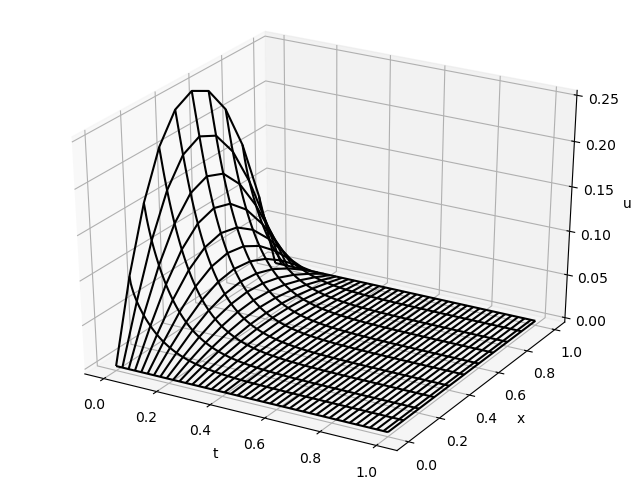
\includegraphics[width=7cm]{img/5-stability1.png}
  \end{center}
  \caption{安定している解}
  \label{fig:stability-1}
 \end{minipage}
 \begin{minipage}{0.5\hsize}
  \begin{center}
   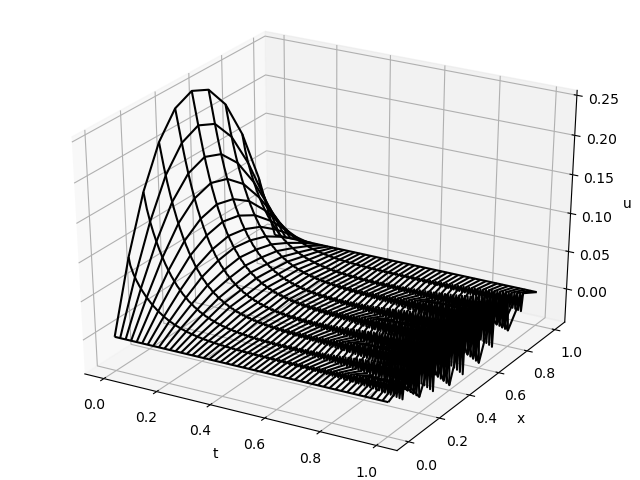
\includegraphics[width=7cm]{img/5-stability2.png}
  \end{center}
  \caption{安定していない解}
  \label{fig:stability-2}
 \end{minipage}
\end{figure}









\section{陰的差分法}
\label{partial-difference-implicit}
陽的差分法では解が安定するために$h$と$k$に条件がありました。それに対し陰的差分法では条件が緩くなったり、完全になくなってしまったりします。

\ref{partial-difference-explicit}節で「陽的差分法で解くには式\ref{eq:partial-difference}の$\alpha$が0である必要がある」と書きました。$\alpha\neq0$のときは$U_{i+1\ j+1}$と$U_{i+1\ j}$の2つの数が未知として1つの式に出てしまうからです。この場合は連立一次方程式\ref{eq:numerical-partial-all}を解くことになります。この行列は疎なので、\ref{gauss-seidel}節で紹介したガウス・ザイデル法などを使って解くことができます。

また、式\ref{eq:partial-difference}で$\alpha=0$である場合にも、差分近似を別のものにしたり、適当に$i$と$j$をずらしたりすることで陰解法に帰着できる場合があります。実際に拡散方程式を解いて確認してみましょう。

陰的差分法で拡散方程式を解くには$\partial u(x,y)/\partial x$および$\partial u(x,y)/\partial y$を後退差分近似に置き換えます。

\begin{eqnarray}
    \frac{\partial}{\partial x}u(x,y)=\frac{u(x,y)-u(x-h,y)}{h}+O(h) \\
    \frac{\partial}{\partial y}u(x,y)=\frac{u(x,y)-u(x,y-k)}{h}+O(k)
\end{eqnarray}

これと\ref{partial-difference-calc}節で紹介した差分近似を代入して、拡散方程式は

\begin{eqnarray}
    \frac{u(t,x)-u(t-h,x)}{h}&=&\frac{u(t,x+k)-2u(t,x)+u(t,x-k)}{k^2} \\
    \frac{U_{i\ j}-U_{i-1\ j}}{h}&=&\frac{U_{i\ j+1}-2U_{i\ j}+U_{i\ j-1}}{k^2}
\end{eqnarray}

\noindent
となります。ここで、$i=i+1$と置換しましょう。

\begin{eqnarray}
    \frac{U_{i+1\ j}-U_{i\ j}}{h}=\frac{U_{i+1\ j+1}-2U_{i+1\ j}+U_{i+1\ j-1}}{k^2} \\
    -\frac{h}{k^2}U_{i+1\ j+1}+\pqty{1+2\frac{h}{k^2}}U_{i+1\ j}-\frac{h}{k^2}U_{i+1\ j-1}=U_{i\ j}
    \label{eq:implicit-diffusion}
\end{eqnarray}

$X$を任意として、左辺にある$U_{i+1\ X}$が未知、右辺の$U_{i\ j}$が未知であるとすると、これは連立一次方程式を解く必要がありそうです。解を求めるのに連立一次方程式を解く必要がある差分法を「陰的差分法」と言います。実際にこれを、陽的差分法で安定しなかったパラメータ$h=0.0052,k=0.1$($h/k^2=0.52$)で解いた結果は図\ref{fig:stability-3}です。また、$h=k=0.1$($h/k^2=10$)でも実験し、図\ref{fig:stability-4}に掲載しました。

\begin{figure}[ht!]
 \begin{minipage}{0.45\hsize}
  \begin{center}
   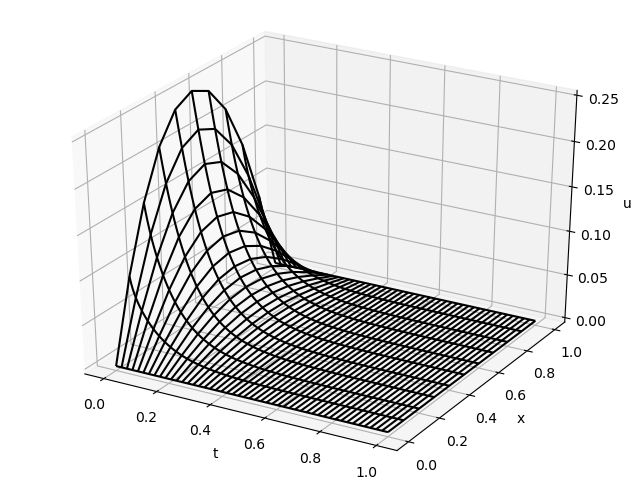
\includegraphics[width=7cm]{img/5-stability3.png}
  \end{center}
  \caption{$h=0.0052,k=0.1$}
  \label{fig:stability-3}
 \end{minipage}
 \begin{minipage}{0.5\hsize}
  \begin{center}
   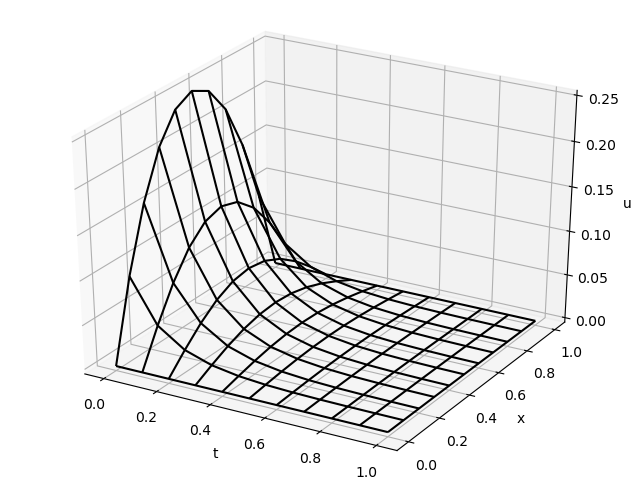
\includegraphics[width=7cm]{img/5-stability4.png}
  \end{center}
  \caption{$h=k=0.1$}
  \label{fig:stability-4}
 \end{minipage}
\end{figure}








\subsection{フォン・ノイマンの安定性解析}
\label{implicit-stability}
では安定性解析を行いましょう。結論から言えば、拡散方程式の場合はどんな$h$と$k$の組み合わせでも解が安定します。

\ref{explicit-stability}節で陽的差分法に対して行ったように、解をフーリエ級数展開し、式\ref{eq:implicit-diffusion}に代入し、\ref{explicit-stability}節と同様に整理します。

\begin{eqnarray}
    -\frac{h}{k^2}C_{l\ i+1}\cos(2\pi lk)+\pqty{1+2\frac{h}{k^2}}C_{l\ i+1}-\frac{h}{k^2}C_{l\ i+1}\cos(2\pi lk)&=&C_{l\ i} \\
    \pqty{1+2\frac{h}{k^2}\pqty{1-\cos(2\pi lk)}}C_{l\ i+1}&=&C_{l\ i}
\end{eqnarray}

半角の公式を使い、$C_{l\ i+1}$について整理すると、

\begin{eqnarray}
    C_{l\ i+1}=\frac{1}{1+4\frac{h}{k^2}\sin^2(\pi lk)}C_{l\ i}
\end{eqnarray}

\noindent
となります。ラックスの同等定理から、

\begin{eqnarray}
    -1\leq\frac{1}{1+4\frac{h}{k^2}\sin^2(\pi lk)}\leq1
\end{eqnarray}

ですが、$0\leq\sin^2(\pi lk)$なので、この式はどんな$h$と$k$の組み合わせに対しても成立します。このことを「無条件安定」と言います。


\end{document}
